\documentclass[10pt]{article}
\usepackage{amsmath,textcomp,amssymb,geometry,graphicx,enumerate,tikz,algorithm,algpseudocode,pifont}
\usetikzlibrary{calc}
\usetikzlibrary{datavisualization}
\usetikzlibrary{datavisualization.formats.functions}


\textheight=9in
\textwidth=7in
\topmargin=-.75in
\oddsidemargin=-0.25in
\evensidemargin=-0.25in

\usepackage{listings}
\lstnewenvironment{codeblock}
    {\lstset{language=Python,
      showspaces=false,
      showtabs=false,
      breaklines=true,
      mathescape=true,
      showstringspaces=false,
      breakatwhitespace=true,
      commentstyle=\textit,
      keywordstyle=\textbf,
      basicstyle=\ttfamily,
      escapechar=`,
      moredelim={**[is][{\color{RoyalBlue}}]{\^^M\\beginsol}{\^^M\\endsol}},
      moredelim={[is][{\color{RoyalBlue}}]{\^^M\\beginexp}{\^^M\\endexp}},
    }}
    {}

\begin{document}
\section*{01/25/2016}
%%%%%%%%%%%%%%%%%%%%%%%%%%%%
\subsection*{Classifiers}
		\ 
		\begin{itemize}
			\item You are given a set of n \underline{samples}, each with d features.

			\item Some samples belong to a certain \underline{class} $\mathcal{O}$; some do not.

			\item Example: sample are bank loans, features are income and age (d=2). Some are in class defaulted; some are not. \underline{Goal}: Predict whether future borrowers will default based on their income and age.

			\item Represent each sample as a point in a d-dimensional space, called a \underline{feature vector} (aka predictors, independent variables).

			\item \underline{Decision boundary}: the boundary chosen by our classifier to separate $\mathcal{O}$ from not $\mathcal{O}$.

			\item Some (not all) classifiers work by computing a \underline{predictor function}: A function $f(x)$ that maps sample point $x$ to a scalar such that,
				\begin{align*}
					& f(x) > 0 \ if \ x \ \in class \ \mathcal{O} \\
					& f(x) \leq 0 \ if \ x \ \notin \ class \ \mathcal{O}\\
				\end{align*}
				(aka decision function, or discriminant function).
				
			\item For these classifiers, the decision boundary is, 
				$$ \{x \in \mathbb{R}^{d}: f(x) = 0 \} $$
				That is the set of all points where the prediction function is zero. Usually this set is a ($d-1$)-dimensional surface in $\mathbb{R}^{d}$.

			\item $\{ x: f(x) = 0 \}$ is also called an \underline{isosurface} (aka isocontours) of $f$ for the \underline{isovalue} 0.

			\item \underline{Linear classifier}: The decision boundary is a hyperplane. Usually uses a linear predictor function.

			\item \underline{Overfitting}: when sinuous (having many curves and turns) decision boundary fits sample data so well that it doesn't classify future (test set) items well.
		\end{itemize}
		
%%%%%%%%%%%%%%%%%%%%%%%%%%%%%%
	\subsection*{Math Review}
		\
		\begin{itemize}
			\item \underline{Vectors}:
			$$
				x = \begin{bmatrix}
 					x_{1} \\
 					x_{2} \\
 					x_{3} \\
 					x_{4} \\
 					x_{5} 
 				\end{bmatrix}
 				= \begin{bmatrix}
 					x_{1} & x_{2} & x_{3} & x_{4} & x_{5}
 				\end{bmatrix}^{T}
			$$
			Think of $x$ as a point in $\mathbb{R}^{d}$.
			
			\item Conventions (often, but not always):
				\begin{itemize}
					\item Uppercase roman = matrix.
					\item Lowercase roman = vector.
					\item Greek = scalar.
					\item Other scalars: n = number of samples, d = number of features or dimension of sample, i, j, and k = indices.
					\item Functions (often scalars): $f()$, $s()$, etc.
				\end{itemize}
			\item \underline{Inner products} (aka dot products)
				\begin{itemize}
					\item $x \cdot y = x_{1}y_{1} + x_{2}y_{2} + \dots + x_{d}y_{d}$
					\item Also written $x^{T}y$.
					\item Clearly, $f(x) = w \cdot x + \alpha$ is a linear function in $x$.
				\end{itemize}
			\item \underline{Eucledian norms}: $||x|| = \sqrt{x \cdot x} = \sqrt{x_{1}^{2} + {x_{2}^{2} + \dots + x_{d}^{2}}}$
				\begin{itemize}
					\item $||x||$ is the length (aka Eucledian length) of a vector $x$.
					\item Given a vector $x$, $\frac{x}{||x||}$ is a unit vector (length 1).
					\item "Normalize" a vector $x$: replace $x$ with  $\frac{x}{||x||}$.
				\end{itemize}
			\item Use dot product to compute angles:\\
				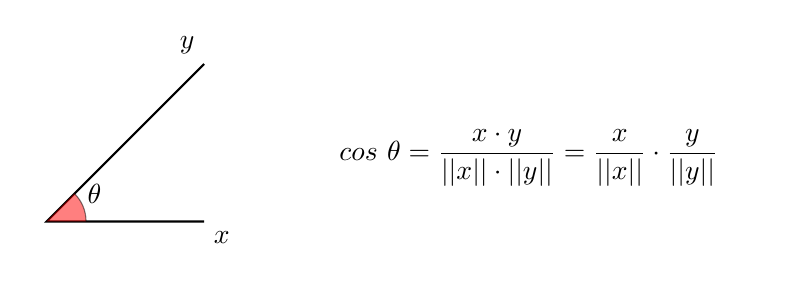
\begin{tikzpicture}
					\coordinate[label=below left:$$] (A) at (0,0);
					\coordinate[label=below right:$x$] (X) at (2,0);
					\coordinate[label=above left:$y$] (Y) at (2,2);

					\draw[thick] (X) -- (A) -- (Y);

					% Mark the angle XAY
					\begin{scope}
					\path[clip] (A) -- (X) -- (Y);
					\fill[red, opacity=0.5, draw=black] (A) circle (5mm);
					\node at ($(A)+(30:7mm)$) {$\theta$};	
					\end{scope}
				\node[text width=6cm, anchor=west, right] at (3,1)
    			{$$cos \ \theta = \frac{x \cdot y}{||x|| \cdot ||y||} = \frac{x}{||x||} \cdot \frac{y}{||y||}$$};
    			\end{tikzpicture}
    			
    			\begin{tikzpicture}
					\coordinate[label=below left:$$] (A) at (0,0);
					\coordinate[label=below right:$$] (X) at (2,0);
					\coordinate[label=above left:$$] (Y) at (2,2);

					\draw[thick] (X) -- (A) -- (Y);

					% Mark the angle XAY
					\begin{scope}
					\path[clip] (A) -- (X) -- (Y);
					\fill[red, opacity=0.5, draw=black] (A) circle (5mm);
					\node at ($(A)+(30:7mm)$) {$\theta$};	
					\end{scope}
				\node[text width=6cm, anchor=west, right] at (3,1)
    			{$$acute, \ cos \ \theta > 0$$};
    			\end{tikzpicture}

    			\begin{tikzpicture}
					\coordinate[label=below left:$$] (A) at (0,0);
					\coordinate[label=below right:$$] (X) at (2,0);
					\coordinate[label=above left:$$] (Y) at (0,2);

					\draw[thick] (X) -- (A) -- (Y);

					% Mark the angle XAY
					\begin{scope}
					\path[clip] (A) -- (X) -- (Y);
					\fill[red, opacity=0.5, draw=black] (A) circle (5mm);
					\node at ($(A)+(30:7mm)$) {$\theta$};	
					\end{scope}
				\node[text width=6cm, anchor=west, right] at (3,1)
    			{$$right, \ cos \ \theta = 0$$};
    			\end{tikzpicture}
    			
    			\begin{tikzpicture}
					\coordinate[label=below left:$$] (A) at (1,0);
					\coordinate[label=below right:$$] (X) at (3,0);
					\coordinate[label=above left:$$] (Y) at (0,2);

					\draw[thick] (X) -- (A) -- (Y);

					% Mark the angle XAY
					\begin{scope}
					\path[clip] (A) -- (X) -- (Y);
					\fill[red, opacity=0.5, draw=black] (A) circle (5mm);
					\node at ($(A)+(30:7mm)$) {$\theta$};	
					\end{scope}
				\node[text width=6cm, anchor=west, right] at (3,1)
    			{$$obtuse, \ cos \ \theta < 0$$};
    			\end{tikzpicture}
    		
    		\item Given a linear predictor function $f(x) = w \cdot x + \alpha$, decision boundary is
				$$ H = \{ x : w \cdot x = - \alpha \} $$
				\begin{itemize}
					\item The set $H$ is called a hyperplane (A line in 2D, a plane in 3D).
				\end{itemize}
				
			\item \underline{Theorem}: Let $\vec{xy}$ be a vector that lies in $H$. Then $w \cdot (y - x) = 0$. \\
				\underline{Proof}: $x$ and $y$ lie on the hyperplane H. $\therefore w \cdot (y - x) = -\alpha - (-\alpha) = 0$.
				
			\item $w$ is called the \underline{normal vector} of $H$. $w$ is normal (perpendicular) or orthogonal to $H$.

			\item If $w$ is a unit vector, $w \cdot x + \alpha$ is called the \underline{signed distance} from $x$ to $H$ i.e. its distance, but positive on one side of $H$; negative on the other. Moreover the distance from $H$ to the origin is $\alpha$. Hence $\alpha = 0$ if and only if $H$ contains the origin.
			
			\item The coefficients in $w$, plus $\alpha$ are called \underline{weights} or \underline{regression coefficients}. Goal of many Machine Learning algorithms is to find what the weights should be.
			
			\item The input data is linearly separable if $\exists$ a hyperplane that separates all samples $\in \mathcal{O}$ from all samples $\notin \mathcal{O}$.
			\end{itemize}

%%%%%%%%%%%%%%%%%%%%%%%%%%%%%%%%
	\subsection*{Perceptron algorithm}
		\
		\begin{itemize}
			\item (Frank Rosenblatt, 1957) Slow, but correct for linearly separable samples. Uses a \underline{numerical optimization} algorithm: \underline{gradient descent}.
			
			\item Consider $n$ sample vectors $x_{1}, x_{2}, \dots x_{n}$.
			
			\item For each sample, let
				\[
 					y_{i} = \left\{\def\arraystretch{1.2}%
 						\begin{array}{@{}c@{\quad}l@{}}
    						1 & \text{if $x_{i} \in \mathcal{O}$}\\
    						-1 & \text{if $x_{i} \notin \mathcal{O}$}\\
  						\end{array}\right.
				\]
			
			\item Goal: find weights $w$ such that
				\begin{align*}
					& x_{i} \cdot w \geq 0 \ \ \ \text{if} \ y_{i} = 1 \\
					& x_{i} \cdot w \leq 0 \ \ \ \text{if} \ y_{i} = -1\\
				\end{align*}
			 
			 \item Equivalently: $y_{i}x_{i} \cdot w \geq 0$. Inequality is called a \underline{constraint}.
			 
			 \item Idea: We define a \underline{risk function} $R$ that is positive if some constraint is violated. Then we use optimization to choose $w$ that minimizes $R$.
			 
			 \item Define the \underline{loss function}
			 	\[
 					L(y, y_{i}) = \left\{\def\arraystretch{1.2}%
 						\begin{array}{@{}c@{\quad}l@{}}
    						0 & \text{if $y_{i}y \geq 0 $}\\
    						-y_{i}y & \text{otherwise}\\
  						\end{array}\right.
				\]
			
			\item Define the \underline{risk function} (aka \underline{objective function} or \underline{cost function})
				$$ R(w) = \sum_{i=1}^{n} L(x_{i} \cdot w, y_{i}) = 
					\sum_{i \in V} -y_{i} \cdot x_{i} \cdot w $$
				where $x_{i} \cdot w$ is our prediction, $y_{i}$ is the correct classification and $v$ is the set of indices $i$ for which $y_{i}x_{i} \cdot w < 0$.
			\item If $w$ classifies $X_{1}, \dots, X_{n}$ correctly, then $R(w) = 0$. Otherwise, $R(w) > 0$; we want to find a better $w$.
			
			\item \textbf{\underline{Goal}: Solve this \underline{optimization problem}; Find $w$ that minimizes $R(w)$.}
	\end{itemize}

\newpage
\section*{01/27/2016}
%%%%%%%%%%%%%%%%%%%%%%%%%%
	\subsection*{Perceptron algorithm continued}
	\
		\begin{itemize}
			\item \underline{Duality} between x-space and w-space:\\
				\begin{center}
					\begin{tabular}{ c|c}
  						x-space (primal) & w-space (dual) \\
  						\hline
  						hyperplan	e: $\{y: w \cdot y = 0\}$ & point: w \\
  						\hline
					\end{tabular}
				\end{center}
				\begin{itemize}
					\item If a point $x \in H$ (hyperplane), then its dual hyperplane $x^{*}$ contains the dual point $H^{*}$ (it also preserves orientation).
				\end{itemize}
			
			\item If we want to enforce inequality $x \cdot w \geq 0$, that means:
				\begin{itemize}
					\item $x$ should be in the correct side of $\{y: y \cdot w = 0\}$ in x-space.
					\item $w$ should be on the correct side of $\{v: x \cdot v = 0\}$ in w-space.
					\item Add image
					\item Note: if data is linearly separable there will always be a section where you can put $w$.
				\end{itemize}
		\end{itemize}

	\subsection*{Optimization algorithm 1} Gradient descent on $R$.
		\begin{itemize}
			\item Given a starting point $w$, find gradient of $R$ with respect to $w$; this is the direction of the steepest ascent. Take a step in the opposite direction.
				\begin{align*}
					& \triangledown R(w) =
						\begin{bmatrix}
 							\frac{\partial R}{\partial w_{1}}\\
 							\frac{\partial R}{\partial w_{2}} \\
 							\vdots \\
 							\frac{\partial R}{\partial w_{d}}
 						\end{bmatrix}
 					\ \ \ \ \text{and} \ \ \ \
 					\triangledown(z \cdot w) =
						\begin{bmatrix}
 							z_{1} \\
 							z_{2} \\
 							\vdots \\
 							z_{d}
 						\end{bmatrix} = z\\
 					& \triangledown R(w) = \sum_{i \in V} \triangledown -y_{i}x_{i} \cdot w = \sum_{i \in V} -y_{i}x_{i}\\
				\end{align*}
			\item At any point $w$, we walk downhill in direction of steepest descent; $- \triangledown R$.
			\end{itemize}
\begin{codeblock}
	Gradient Descent:
	    $w \leftarrow$ arbitrary non-zero starting point (good choice is any $y_{i}x_{i}$)
	    while ($R(w) > 0$):
	        $V \leftarrow$ the set of indices $i$ for which $y_{i}x_{i} \cdot w < 0$
	        $w \leftarrow w + \epsilon \sum_{i \in V} y_{i}x_{i}$
\end{codeblock}
			\begin{itemize}
			\item Here $\epsilon$ is the step size (aka learning rate chosen empirically).
			
			\item Problem: Slow! Each step takes $\mathcal{O}(nd)$ time.
		\end{itemize}
	
	\subsection*{Optimization algorithm 2} Stochastic gradient descent
		\
		\begin{itemize}
			\item Idea: Each step, pick \underline{one} misclassified $x_{i}$; do gradient descent on loss function $L(x_{i} \cdot w, y_{i})$.
			\item Called perceptron algorithm. Each step takes $\mathcal{O}(d)$ time.
			\end{itemize}
\begin{codeblock}
	Perceptron Algorithm:
	    while (some $y_{i}X_{i} < 0$):
		    $w \leftarrow w + \epsilon y_{i}x_{i}$
\end{codeblock}
		\begin{itemize}
		\item What if separating hyperplane doesn't pass through the origin?
			\begin{itemize}
				\item Add a fictitious dimension.
				\item Hyperplane: $w \cdot x + \alpha = 0$,
					$$
						\begin{bmatrix} w_{1} & w_{2} & \dots & w_{d} & \alpha \end{bmatrix}
						\begin{bmatrix}
 							x_{1} \\
 							x_{2} \\
 							\vdots \\
 							x_{d}	\\
 							1
 						\end{bmatrix}
					$$
				\item Now we have samples in $\mathbb{R}^{d+1}$, all lying on plane $X_{d+1} = 1$.
			\end{itemize}
		
		\item Perceptron Convergence Theorem: If data is linearly separable, perceptron algorithm finds a correct linear classifier in at most $\mathcal{O}(\frac{R^{2}}{\gamma^{2}})$ iterations; where $R = \max |X_{i}|$ is the "radius of data" and $\gamma$ is the "margin"  (length of longest feature vector).
		\end{itemize}
		
	\subsection*{Maximum Margin Classifiers}
		\
		\begin{itemize}
			\item The margin of a linear classifier is the distance from the decision boundry to the nearest sample.
			\item Lets make the margin as big as possible.
				\begin{center}
					\begin{tikzpicture}
					\datavisualization [school book axes,
                    	visualize as smooth line,
                   		y axis={},
                   		x axis={label}]
						data [format=function] {
      					var x : interval [-3:3] samples 2;
      					func y = \value x*-1;
      					};
      					data [format=function] {
      					var x : interval [-3:3] samples 2;
      					func y = \value x*-1 + 2;
     					};
					\end{tikzpicture}
				\end{center}
			\item We enforce constraints $y_{i}(w \cdot x_{i} + \alpha) \geq 1 \ \ \forall i \in [1, n]$.
			\item If $||w|| = 1$, constraints imply the margin is at least 1.
			\item But we allow to have any length, so the margin is at least $\frac{1}{||w||}$.
			\item There is a \underline{slab} of width $\frac{2}{||w||}$ that contains no samples.
			\item To maximize the margin, minimize $||w||$.
			\item Optimization Problem:
				\begin{center}
					Find $w$ and $\alpha$ that maximize $||w||^{2}$ subject to $y_{i}(w \cdot x_{i} + \alpha) \geq 1 \ \ \forall i \in [1, n]$.
				\end{center}
			\item This is called a \underline{quadratic program} in $d+1$ dimensions and $n$ constraints.
			\item It has one unique solution!
			\item The solution gives us a \underline{maximum margin classifier}, aka a \underline{hard margin support vector machine} (SVM).
		\end{itemize}

\newpage
\section*{02/08/2016}
	\subsection*{Decision Theory}
	\
	\begin{itemize}
		\item Multiple samples with different classes could lie on the same point.
		\item We want a probabilistic classifier.
		\item Suppose 10\% of the population has cancer; 90\% doesn't. We have a probability distribution for calorie intake, $P(X|Y)$:
		\begin{center}
			\begin{tabular}{| c | c | c | c |}
				\hline
 				Calories(X) & $< 1200$ & $1200 - 1600$ & $> 1600$\\
 				\hline
 				Cancer (Y=1) & 20\% & 50\% & 30\%\\
 				\hline
 				no cancer (Y=-1) & 1\% & 10\% & 89\%\\
 				\hline
			\end{tabular}
		\end{center}
	
		\item Recall: $P(X) = P(X|Y=1)P(Y=1) + P(X|Y=-1)P(Y=-1)$
		\item $P(1200 \leq X \leq 1600) = 0.5\cdot 0.1 + 0.1\cdot 0.9 = 0.14$
		\item You meet guy eating $x = 1400$ cals/day. Guess whether he has cancer?
		\item \textbf{Bayes' Theorem}:
			\begin{align*}
				P(A=a|B) &= \frac{P(B|A=a)P(A=a)}{P(B)}\\
				P(Y=1|X=1400) &= \frac{P(X=1400|Y=1)P(Y=1)}{P(X=1400)} = \frac{0.05}{0.14} \\
				P(Y=-1|X=1400) &= \frac{P(X=1400|Y=-1)P(Y=-1)}{P(X=1400)} \frac{0.09}{0.14} \\
				P(Y=1|X=1400) &= \frac{5}{14} \approx 36\% \ \text{probability guy with 1400 cal/day has cancer}\\
			\end{align*}
		\item A \underline{loss function} $L(z, y)$ specifies badness if true class is $y$; classifier prediction is $z$.
			\[
 				L(z, y) = \left\{\def\arraystretch{1.2}%
 					\begin{array}{@{}c@{\quad}l@{}}
    					1 & \text{if $z=1, y=-1$}\\
   						5 & \text{if $z=-1, y=1$}\\
   						0 & \text{otherwise}\\
						\end{array}\right.
			\]
		\item Definitions: 
			\begin{itemize}
				\item loss function above is \underline{asymmetrical}
				\item The \underline{0-1 loss function} is 1 for incorrect predictions, 0 for correct.
			\end{itemize}
		\item Let $r: \mathbb{R}^{d} \rightarrow \pm 1$ be a \underline{decision rule}, aka \underline{classifier}: a function that maps a feature vector $x$ to 1 ("in class") or -1 ("not in class").
		\item The \underline{risk} for $r$ is the expected loss over all values of $x,y$:
			\begin{align*}
				R(r) &= E[L(r(X), Y)]\\
					&= \sum_{x} (L(r(x), 1)P(Y=1|X=x) + L(r(x), -1)P(Y=-1|X=x))P(x)\\
					&= \sum_{x} (L(r(x), 1)\frac{P(X=x|Y=1)(P(Y=1)}{P(x)} 
							+ L(r(x), 1)\frac{P(X=x|Y=-1)(P(Y=-1)}{P(x)})P(x)\\
					&= P(Y=1)\sum_{x} L(r(x), 1)P(X=x|Y=1) +
						P(Y=-1)\sum_{x} L(r(x), -1)P(X=x|Y=-1)\\
			\end{align*}
		\item The \underline{Bayes optimal decision rule} aka \underline{Bayes classifier} is the $r$ that minimizes $R(r)$; call it $r^{*}$. Assuming $L(z, y) = 0$ for $z=y$:
			\[
 				r^{*}(x) = \left\{\def\arraystretch{1.2}%
 					\begin{array}{@{}c@{\quad}l@{}}
    					1 & \text{if $L(-1,1)P(Y=1|X=x) > L(1,-1)P(Y=-1|X=x$)}\\
   						-1 & \text{otherwise}\\
						\end{array}\right.
			\]
		\item In cancer example, $r^{*} = 1$ for all intakes $\leq 1600$; $r^{*} = -1$ for intakes $\geq 1600$, then the \underline{Bayes risk}, aka \underline{optimal risk} is:
		\begin{align*}
			R(r^{*}) = 0.1(5\cdot 0.3) + 0.9(1 \cdot 0.01 + 1 \cdot 0.1) = 0.249\\
		\end{align*}
		\item Suppose $X$ has a continuous probability density function (PDF):
		\item Review:
			\begin{itemize}
				\item probability that random variable
				$X \in [x_{1}, x_{2}] = \int_{x_{1}}^{x_{1}} P(x) dx$\\
				\item area under whole curve $\int_{-\infty}^{\infty} P(x) dx = 1$\\
				\item \underline{expected} value of $f(x): E[f(x)] = \int_{-\infty}^{\infty} f(x)P(x) dx$\\
				\item \underline{mean} $\mu = E[x] = \int_{-\infty}^{\infty} xP(x) dx$\\
				\item \underline{variance} 
					$\sigma^{2} = E[(X-\mu)^{2}] = E[X^{2}] - \mu^{2}$\\
					\begin{center}
						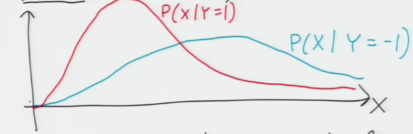
\includegraphics[scale=0.5]{images/gaus}
					\end{center}
				\item Suppose $P(Y=1) = \frac{1}{3}$, $P(Y=-1) = \frac{2}{3}$.
					\begin{center}
						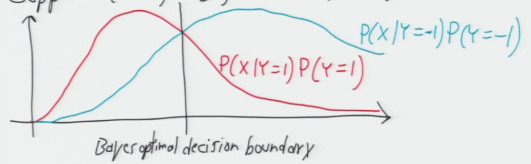
\includegraphics[scale=0.5]{images/othrgaus}
					\end{center}
			\end{itemize}
		\item Define \underline{risk} as before, replace summations with integrals.
			\begin{align*}
				R(r) &= E[L(r(X), Y)]\\
					&= \int_{x} (L(r(x), 1)P(Y=1|X=x) + L(r(x), -1)P(Y=-1|	X=x))P(x)dx\\
					&= P(Y=1)\int_{x} L(r(x), 1)P(X=x|Y=1)dx +
					P(Y=-1)\int_{x} L(r(x), -1)P(X=x|Y=-1)dx\\
			\end{align*}
		\item If $L$ is 0-1 loss, $R(r) = P(r(x)) \ \text{is wrong}$\\
		\item For Bayes decision rule, Bayes Risk is the area under the minimum of the functions above. Assuming $L(z,y) = 0$ for $x=y$:
			\begin{align*}
			R(r^{*}) = \int min_{y \pm 1} L(-y, y)P(X=x|Y=y)P(Y=y)dx\\
			\end{align*}
		\item \underline{Bayes optimal decision boundary}: $\{x: P(Y=1|X=x) = 0.5\}$.
			\begin{center}
				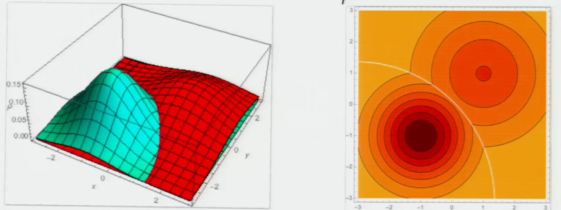
\includegraphics[scale=0.5]{images/cancergaus}
			\end{center}
	\end{itemize}
	
	\subsection*{3 Ways to Build Classifiers}
	\
		\begin{enumerate}
			\item Generative models (e.g. LDA)
				\begin{itemize}
					\item Assume samples come from probability distributions, different for each class.
					\item Guess form of distributions.
					\item For each class C, fit distribution parameters for class C samples, giving $P(X|Y=C)$.
					\item For each C, estimate $P(Y=C)$.
					\item Bayes' Theorem gives $P(Y|X)$.
					\item If 0-1 loss, pick class C that maximizes $P(Y=C|X=x)$. Equivalently, maximizes $P(X=x|Y=C)P(Y=C)$.
				\end{itemize}
			\item Discriminative models (e.g. logistic regression)
				\begin{itemize}
					\item Model $P(Y|X)$ directly 
				\end{itemize}
			\item Find decision boundary (e.g. SVM).
				\begin{itemize}
					\item Model $r(x)$ directly (no posterior).
				\end{itemize}
		\end{enumerate}
		
		\begin{itemize}
			\item Advantages of (1, 2): $P(Y|X)$ tells you probability your guess is wrong.
			\item Advantage of (1): you can diagnose outliers: $P(x)$ is very small.
			\item Disadvantages of (1): often hard to estimate distribution accurately; real distributions rarely match standard ones.
		\end{itemize}

\newpage
\section*{02/10/2016}
	\subsection*{Gaussian Discriminant Analysis}
		\
		\begin{itemize}
			\item Fundamental assumption: each class comes from a normal distribution (Gaussian).
				\begin{align*}
					X \sim \mathcal{N}(\mu, \sigma^{2}):
					P(X) = \frac{1}{\sqrt{2\pi}\sigma} e^{-\frac{|x-\mu|^{2}}{2\sigma^{2}}}\\ 
				\end{align*}
			\item For each class c, suppose we estimate mean $\mu_{c}$, variance $\sigma_{c}^{2}$, and prior $\pi_{c} = P(Y=c)$.
			\item Given $x$, Bayes' rule $r^{*}(x)$ return class C that maximizes $P(X=x|Y=c)\pi_{c}$.
			\item $\ln z$ is monotonically increasing for $z > 0$, so its equivalent to maximize,
				\begin{align*}
					Q_{c}(x) &= \ln(\sqrt{2\pi}P(X=c|Y=c)\pi_{c})\\
							&= -\frac{|x-\mu_{c}|^{2}}{2\sigma^{2}} - \ln \sigma_{c} + \ln \pi_{c}\\
				\end{align*}
			\item $Q_{c}(x)$ is quadratic in $x$.
		\end{itemize}
	
	\subsection*{Quadratic Discriminant Analysis (QDA)}
		\
		\begin{itemize}
			\item Suppose only 2 classes c, d, Then,
				\[
 				r^{*}(x) = \left\{\def\arraystretch{1.2}%
 					\begin{array}{@{}c@{\quad}l@{}}
    					c & \text{if $Q_{c}(x) - Q_{d}(x) > 0$}\\
   						d & \text{otherwise}\\
					\end{array}\right.
				\]
			\item The $Q_{c}(x) - Q_{d}(x)$ prediction function is quadratic in $x$.
			\item Bayes decision boundary is $Q_{c}(x) - Q_{d}(x) = 0$.
			\item In 1D, Bayesian decision boundary may have 1 or 2 points.
			\item In d-D, Bayesian decision boundary is a quadric. 
			\item To recover posterior probabilities in 2-class case, use Bayes:
				\begin{align*}
					P(Y=c|X) = \frac{P(X|Y=c)\pi_{c}}{P(X|Y=c)\pi_{c} + P(X|Y=d)\pi_{d}}
				\end{align*}
			\item Recall $e^{Q_{c}(x)} = \sqrt{2\pi}P(x)\pi_{c}$.
				\begin{align*}
					P(Y=c|X=x) &= \frac{e^{Q_{c}(x)}}{e^{Q_{c}(x)} + e^{Q_{d}(x)}}\\
					&= \frac{1}{1 + e^{Q_{c}(x) - Q_{d}(x)}}\\
					&= s(Q_{c}(x) - Q_{d}(x))
				\end{align*}
			\item Where s($\cdot$) is the \underline{logistic function} aka \underline{sigmoid function}, 
				\begin{align*}
					s(\gamma) = \frac{1}{1 + e^{-\gamma}}\\
				\end{align*}
				\begin{itemize}
					\item Monotonically increasing.\\
					\item $s(0) = \frac{1}{2}$.\\
					\item $s(\infty) \rightarrow 1$.\\
					\item $s(-\infty) \rightarrow -1$.\\
					\item always $\in [0, 1] \rightarrow$ probabilities.
				\end{itemize}
		\end{itemize}
		
	\subsection*{Linear Discriminant Analysis (LDA)}
		\
		\begin{itemize}
			\item Fundamental assumption: all the Gaussians have the same variance $\sigma$ only difference between classes is the mean $\mu_{i}$.
			\item Then,
				\begin{align*}
					Q_{c}(x) - Q_{d}(x) = \frac{(\mu_{c}-\mu_{d})\cdot x}{\sigma^{2}} - \frac{\mu_{c}^{2}-\mu_{d}^{2}}{2\sigma^{2}} + \ln \pi_{c} + \ln \pi_{d}\\
				\end{align*}
			\item Now its a linear classifiers! Choose c that maximizes,
				\begin{align*}
					\frac{\mu_{c}\cdot x}{\sigma^{2}} - \frac{\mu_{c}^{2}}{2\sigma^{2}} + \ln \pi_{c}\\
				\end{align*}
			\item In 2-class case, decision boundary is $w \cdot x + \alpha = 0$.
			\item If $\pi_{c} = \pi_{d} = \frac{1}{2} \implies (\mu_{c} - \mu_{d})\cdot x - \frac{(\mu_{c}-\mu_{d})}{2} = 0$
			\item This is the centroid method!
			\item In 2-class case, Bayes posterior is $P(Y=c|X=x) = s(w\cdot x + \alpha)$
		\end{itemize}
	
	\subsection*{Maximum Likelihood Estimation of Parameters} (Ronald Fisher, circa 1912)
		\
		\begin{itemize}
			\item Lets flip biased coins. Heads with probability $p$; tails with probability $1-p$.
			\item 10 flips, 8 heads, 2 tails. What is the most likely value of $p$?
			\item Binomial Distribution: $X \sim B(n, p)$
				\begin{align*}
					P[X=x] = {n \choose x} p^{x}(1-p)^{n-x}\\
				\end{align*}
			\item Our example: n=10,
				\begin{align*}
					P[X=10] = 45 p^{8}(1-p)^{2} = \mathcal{L}(x)\\
				\end{align*}
			\item Probability of 8 heads in 10 flips: written as a function $\mathcal{L}(p)$ of distribution parameter(s); this is the \underline{likelihood function}
			\item \underline{Maximum likelihood estimation} (MLE): A method of estimating parameters of a statistical model by picking the parameters that maximize the likelihood function.
				\begin{center}
					\begin{tabular}{| c |}
						\hline
 					Find $p$ that maximizes $\mathcal{L}(p)$\\
 					\hline
					\end{tabular}
				\end{center}
			\item Solve this example by setting derivative equal to 0:
				\begin{align*}
					\frac{d\mathcal{L}}{dp} &= 360p^{7}(1-p)^{2} - 90p^{8}(1-p) = 0\\
						&\implies 4(1-p)-p = 0 \implies p=0.8\\
				\end{align*}
			\item The \underline{log likelihood} $\mathcal{L}(\cdot)$ is the $\ln$ of the likelihood $\mathcal{L}(\cdot)$.
		\end{itemize}
	
	\subsection*{Likelihood of a Gaussian}
		\
		\begin{itemize}
			\item Given samples $x_{1}, x_{2}, \dots, x_{n}$ find best-fit Gaussian.
			\item Likelihood of generating these samples is,
				\begin{align*}
					\mathcal{L}(\mu, \sigma;x_{1}, \dots, x_{n}) = P(x_{1})P(x_{2}) \dots P(x_{n})\\
				\end{align*}
			\item Log likelihood is,
				\begin{align*}
					l(\mu, \sigma) = \sum_{i=1}^{n} \ln P(x_{i})
				\end{align*}
			\item Want to set $\triangledown_{\mu} l = 0$, and  $\frac{\partial l}{\partial \sigma} = 0$.
			\item Natural log of Gaussian distribution,
				\begin{align*}
					\ln P(x) = -\frac{|x-\mu|^{2}}{2\sigma^{2}} - \ln \sqrt{2\pi} - \ln \sigma\\
				\end{align*}
			\item taking the gradient,
				\begin{align*}
					\triangledown_{\mu}l = \sum_{i} \frac{x_{i}-\mu}{\sigma^{2}} &\implies \hat{\mu} = \frac{1}{n} \sum_{i} x_{i}\\
					\frac{\partial l}{\partial \sigma} = \sum_{i} \frac{|x_{i} - \mu|^{2} - \sigma^{2}}{\sigma^{3}} = 0 &\implies \hat{\sigma^{2}} = \frac{1}{n} \sum_{i} |x_{i} - \mu|^{2}\\
				\end{align*}
			\item We don't know $\mu$ exactly, so substitute $\hat{\mu}$ in the last equation above.
			\item For QDA: estimate mean and variance of each class as above, and estimate the priors (for each class c):
				\begin{align*}
					\hat{\pi_{c}} = \frac{n_{c}}{\sum_{d} n_{d}} \leftarrow \ \text{denominator is the sum of samples in all classes}
				\end{align*}
			\item For LDA: same mean and priors; one variance for all classes:
				\begin{align*}
					\hat{\sigma^{2}} = \frac{1}{n} \sum_{c} \sum_{i:y_{i}=c} |x_{i} - \mu_{c}|^{2}
				\end{align*}
		\end{itemize}

\newpage
\section*{02/17/2016}
	\subsection*{Eigenvectors}
	\
		\begin{itemize}
			\item Given a matrix A, if $Av = \lambda v$ for some vector $v \neq 0$, scalar $\lambda$, then $v$ is an \underline{eigenvector} of A and $\lambda$ is the associated \underline{eigenvalue} of A.
			
				\begin{center}
					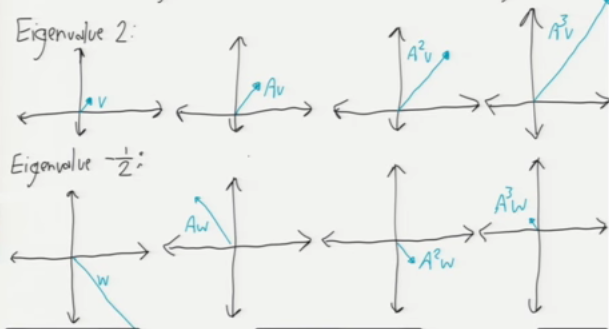
\includegraphics[scale=0.5]{images/eigenvectors}
				\end{center}
			\item Theorem: if $v$ is an eigenvector of A with eigenvalue $\lambda$, then $v$ is an eigenvector of $A^{k}$ with eigenvalue $\lambda^{k}$.
			\item Proof: $A^{2}v = A(\lambda v) = \lambda^{2}v$ etc.
			\item Theorem: moreover, if $A$ is invertible, then $v$ is an eigenvector of $A^{-1}$ with eigenvalue $\frac{1}{\lambda}$.
			\item Proof: $A^{-1}v = \frac{1}{\lambda}A^{-1}Av = \frac{1}{\lambda}v$.
			\item \underline{Spectral Theorem}: Every symmetric $nxn$ matrix has $n$ eigenvectors that are mutually orthogonal,
				\begin{align*}
					v_{i}^{T}v_{j} = 0, \forall i\neq j
				\end{align*}
			\item We can use them as a basis for $\mathbb{R}^{n}$.
				\begin{center}
					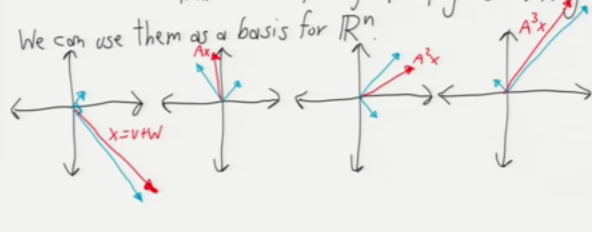
\includegraphics[scale=0.5]{images/basis}
				\end{center}
			\item Write $x$ as a linear combination of eigenvectors:
				\begin{align*}
					x &= \alpha v + \beta w\\
					A^{k}x &= \alpha \lambda_{v}^{k} v + \beta \lambda_{w}^{k} w\\
				\end{align*}
			\item \underline{Ellipsoids}
				\begin{align*}
					f(x) &= x^{T}x \Leftarrow \text{quadratic; isotropic; isosurfaces are spheres.}\\
					g(x) &= f(Ax) \Leftarrow A \text{symmetric}.\\
					  	&= x^{T}A^{2}x \Leftarrow\text{\underline{quadratic form} of the matrix} \ A^{2} \ \text{anisotropic; isosurfaces are ellipsoids}\\
				\end{align*}
				\begin{center}
					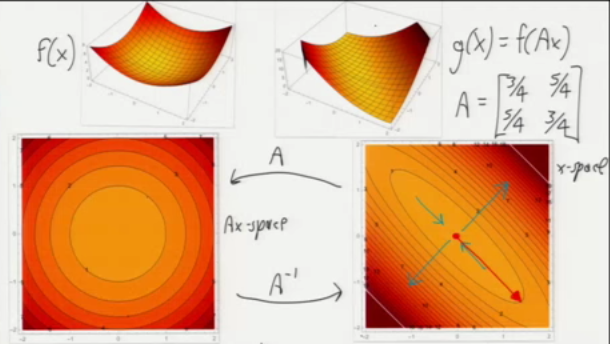
\includegraphics[scale=0.7]{images/ellipses}
				\end{center}
				\begin{itemize}
					\item $g(x) = 1$ is an ellipsoid with axes $v_{1}, v_{2}, \dots, v_{n}$  and radii $\frac{1}{\lambda_{1}}, \frac{1}{\lambda_{2}}, \dots, \frac{1}{\lambda_{n}}$ (eigevalues of A) because if $v_{i}$ has length $\frac{1}{\lambda_{i}}$ (red arrow), $g(v_{i}) = f(\lambda_{i}v_{i}) = 1 \Rightarrow v_{i}$ lies on the ellipsoid.
				\end{itemize}
			\item Bigger eigenvalue $\Leftrightarrow$ steeper slope $\Leftrightarrow$ shorter ellipsoid radius.
			\item Alternative interpretation:
				\begin{itemize}
					\item Ellipsoids are spheres in a \unexpanded{distance metric} $A^{2}$.
					\item Call $M = A^{2}$ a \underline{metric tensor} because the distance between samples $x$ and $z$ in stretched space is $d(x, z) = |Ax - Az| = \sqrt{(x-z)^{T}M(x-z)}$.
					\item Ellipsoids are "spheres" in this metric: $\{x: d(x, \text{center}) = \text{isovalue}\}$.
				\end{itemize}
			\item A square matrix $B$ is,
				\begin{itemize}
					\item \underline{positive definite} if $w^{T}Bw > 0$ for all $w \neq 0 \Leftrightarrow$ all positive eigenvalues.
					\item \underline{positive semidefinite} if $w^{T}Bw \geq 0$ for all $w \neq 0 \Leftrightarrow$ all non-eigenvalues.
					\item \underline{indefinite} if at least one positive eigenvalue and one negative eigenvalue.
					\item \underline{invertible} if no zero eigenvalue.
					\begin{center}
						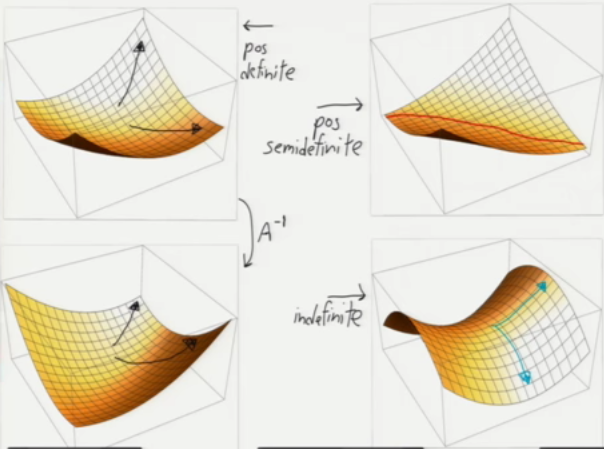
\includegraphics[scale=0.5]{images/matrices}
					\end{center}
				\end{itemize}
			\item Metric tensor must be symmetric positive definite (SPD).
			\item Special case: $M$ and $A$ are diagonal matrices $\Leftrightarrow$ eigenvectors are coordinate axes $\Leftrightarrow$ ellipsoids are axis-aligned.
		\end{itemize} 
	
	\subsection*{Building a Quadratic with specified eigenvectors and eigenvalues}
		\
		\begin{itemize}
			\item Choose $n$ mutually orthogonal unit n-vectors $v_{1}, \dots, v_{n}$ Let, $V = [v_{1}, v_{2}, \dots, v_{n}]$
			\item Observe: $V^{T}V = I \Rightarrow V^{T} = V^{-1} \Rightarrow VV^{T} = I$.
			\item $V$ is \underline{orthogonal matrix}: acts like rotation (or reflection).
			\item Choose some inverse radii $\lambda_{i}$:
			\item Let,
				\begin{align*}
					\Lambda =
						\begin{bmatrix}
							\lambda_{1} & 0 & \dots & 0\\
							0 & \lambda_{2} & \dots & 0\\
							\vdots & & \ddots & \vdots &\\
							0 & 0 & \dots & \lambda_{n}\\
						\end{bmatrix}
				\end{align*}
			\item Theorem: $A = V\Lambda V^{T} = \sum_{i=1}^{n} \lambda_{i} v_{i}v_{i}^T$ has chosen eigenvectors and eigenvalues.
			\item Proof: $AV = V\Lambda \Leftarrow$ definition of eigenvectors! (in matrix form).
			\item This is a \underline{matrix factorization} called the \underline{eigen-decomposition}
			\item $\Lambda$ is the diagonalized version of $A$.
			\item $V^{T}$ rotates the ellipsoid to be axis-aligned.
			\item This is also a recipe for building quadratics with axes $v_{i}$, radii $\frac{1}{\lambda_{i}}$.
			\item Given SPD metric tensor M, we can find symmetric \underline{square root} $A = M^{\frac{1}{2}}$:
				\begin{itemize}
					\item compute eigenvectors and eigenvalues of $M$
					\item take square roots of $M's$ eigenvalues
					\item reassemble matrix $A$.
				\end{itemize}
		\end{itemize}

\newpage
\section*{02/22/2016}
	\subsection*{Anisotropic Multivariate Gaussians}
		\
		\begin{itemize}
			\item $X \sim \mathcal{N}(\mu, \Sigma) \Leftarrow X$ is random d-vector with mean $\mu$.
				\begin{align*}
					P(x) &= \frac{1}{\sqrt{(2\pi)^{d}}\sqrt{|\Sigma|}}\text{exp}(-\frac{1}{2}(x-\mu)^{T}\Sigma^{-1}(x-\mu))
				\end{align*}
			\item $\Sigma$ is the $d$x$d$ SPD \underline{covariance matrix}
			\item $\Sigma^{-1}$ is the $d$x$d$ SPD \underline{precision matrix}; serves as a metric tensor.
			\item Write $P(x) = n(q(x))$, where $q(x) = (x-\mu)^{T}\Sigma^{-1}(x-\mu)$. Note, $n: \mathbb{R} \rightarrow \mathbb{R}$, exponential, $q: \mathbb{R}^{d} \rightarrow \mathbb{R}$, quadratic.
			\item Principle: given $f: \mathbb{R} \rightarrow \mathbb{R}$, isosurfaces of $f(q(x))$ are same as $q(x)$ (different isovalues), except that some might be "combined."
				\begin{center}
					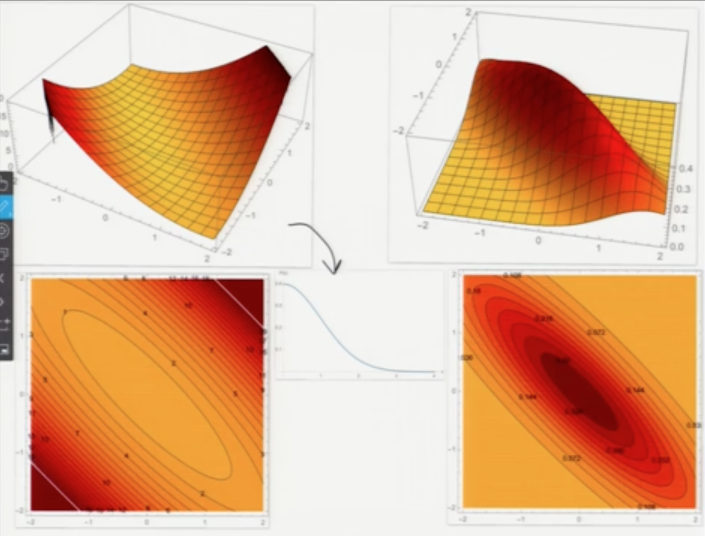
\includegraphics[scale=0.5]{images/gaussiantransformation}
				\end{center}
			\item \underline{Covariance}:
				\begin{align*}
					\text{Cov}(X, Y) &= E[(X - E[X])(Y - E[Y])^{T}]\\
									&= E[XY^{T}] - \mu_{x}\mu_{y}^{T}\\
					\text{Var}(X) &= \text{Cov}(X, X)\\
				\end{align*}
				\begin{itemize}
					\item For a Gaussian, one can show Var($X$) = $\Sigma$. Hence,
						\begin{align*}
							\Sigma =
								\begin{bmatrix}
									\text{Var}(X_{1}) & \text{Cov}(X_{1},X_{2}) & \dots & \text{Cov}(X_{1},X_{d})\\
									\text{Cov}(X_{2},X_{1})  & \text{Var}(X_{2}) & \dots & \text{Cov}(X_{2}, X_{d})\\
									\vdots & & \ddots & \vdots &\\
									\text{Cov}(X_{d},X_{1}) & \text{Cov}(X_{d},X_{2}) & \dots & \text{Var}(X_{d})\\
								\end{bmatrix}
						\end{align*}	
					\item $X_{i}, X_{j}$ independent $\Rightarrow$ Cov($X_{i}, X_{j}$) = 0.
					\item Cov($X_{i}, X_{j}$) = 0 and they come from a joint normal distribution $\Rightarrow X_{i}, X_{j}$ independent.
					\item All features pairwise independent $\Rightarrow \Sigma$ is diagonal.
						\begin{align*}
							\Sigma \ \text{is diagonal} &\Leftrightarrow \text{axis-aligned Gaussian; squared radii on the diagonal}.\\
							&\Leftrightarrow P(x) = P(X_{1})P(X_{2}) \dots P(X_{d})\\
						\end{align*}

\begin{center}						
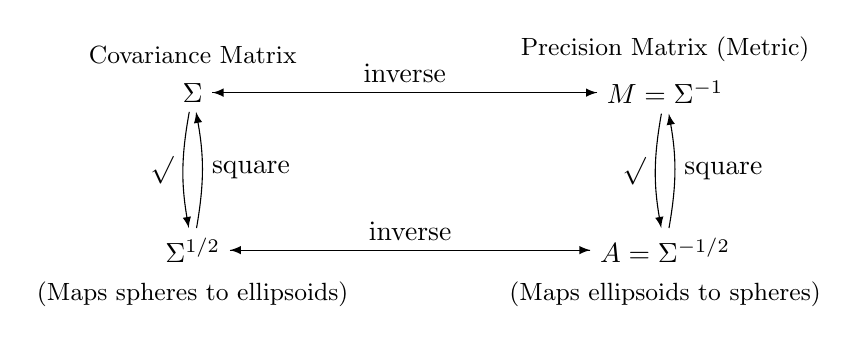
\begin{tikzpicture}
[ar/.style={->,thick},no/.style={}]
\node [no][label={\small Covariance Matrix}] at (0cm,4cm) (A) {$\Sigma$};
\node [no][label={\small Precision Matrix (Metric)}] at (6cm,4cm) (B) {$M = \Sigma^{-1}$};
\node [no][label=below:{\small (Maps ellipsoids to spheres)}] at (6cm,2cm) (D) {$A=\Sigma^{-1/{2}}$};
\node [no][label=below:{\small (Maps spheres to ellipsoids)}] at (0cm,2cm) (E) {$\Sigma^{1/{2}}$};

\draw [-latex] (A) -- node[above] {inverse} (B);
\draw [-latex] (B) -- node[above] {} (A);

\draw [-latex] (A) to[bend right=10] node[left] {$\sqrt{}$} (E);
\draw [-latex] (E) to[bend right=10] node[right] {square} (A);

\draw [-latex] (B) to[bend right=10] node[left] {$\sqrt{}$} (D);
\draw [-latex] (D) to[bend right=10] node[right] {square} (B);


\draw [-latex] (D) -- node[above] {inverse} (E);
\draw [-latex] (E) -- node[above] {} (D);
\end{tikzpicture}
\end{center}	
					\item Eigenvalues of $\Sigma^{1/{2}}$ are ellipsoid radii (standard deviations along the eigenvectors).
					\item Eigenvalues of $\Sigma$ are variances along along eigenvectors.
					\item Diagonalizing $\Sigma = V\Lambda V^{T}$, $\Sigma^{\frac{1}{2}} = V\Lambda^{\frac{1}{2}}V^{T}$.
				\end{itemize}
			\end{itemize}
		
		\subsection*{Maximum Likelihood estimation for anisotropic Gaussians}
			\
			\begin{itemize}
				\item Given samples $x_{1}, \dots, x_{n}$ and classes $y_{1}, \dots y_{n}$ find the best-fit Gaussians.
				\item For QDA:
					\begin{align*}
						\hat{\Sigma_{c}} = \frac{1}{n_{c}} \sum_{i:y_{i}=c} (x_{i} - \mu_{c})(x_{i} - \mu_{c})^{T} \Leftarrow \text{conditional covariance for samples in class c}
					\end{align*}
					\begin{center}
						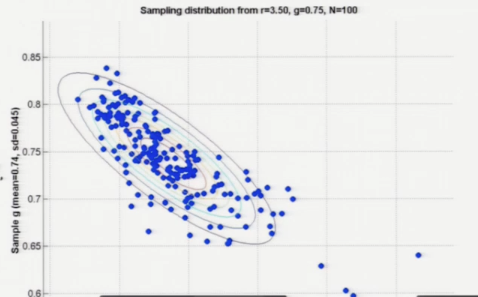
\includegraphics[scale=0.5]{images/smaple}
					\end{center}
					\begin{itemize}
					\item Priors $\pi_{c}$ and means $\hat{\mu_{c}}$ same as before.
					\item $\hat{\Sigma_{c}}$ is the positive semidefinite. If some zero eigenvalue, must eliminate the zero-variance dimension.
					\end{itemize}
				\item For LDA:
					\begin{align*}
						\hat{\Sigma} = \frac{1}{n} \sum_{c} \sum_{i:y_{i}=c} (x_{i} - \mu_{c})(x_{i} - \mu_{c})^{T} \Leftarrow \text{pooled within class covariance matrix}
					\end{align*}
				\item \underline{QDA}:
					\begin{itemize}
						\item $\pi_{c}, \mu_{c}, \Sigma_{c}$ may be different for each class c.
						\item Goal is to choose c that maximizes $P(X=x|Y=c)\pi_{c}$ , which is equivalent to maximizing the \underline{quadratic discriminant function},
							\begin{align*}
								Q_{c}(x) &= \ln \Big(\sqrt{(2\pi)^{d}}P(x)\pi_{c}\Big)\\
										&= -\frac{1}{2}q_{c}(x)-\frac{1}{2} \ln |\Sigma_{c}| + \ln \pi_{c}
							\end{align*}
						\item 2 classes: Prediction function $Q_{c}(x) - Q_{d}(x)$ is quadratic, but may be indefinite.
						\item Since the prediction function is quadratic $\Rightarrow$ Bayes decision boundary is quadric.
						\item Posterior is $P(Y=c|X=x) = s(Q_{c}(x) - Q_{d}(x))$ where $s(\cdot)$ is the logistic function.
							\begin{center}
								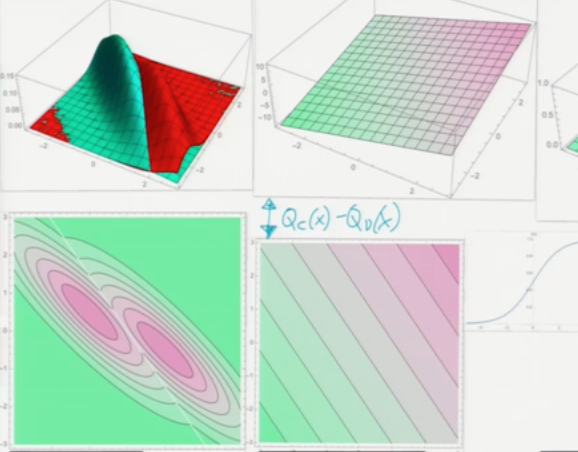
\includegraphics[scale=0.5]{images/LDA}
							\end{center} 
					\end{itemize}
				
				\item \underline{LDA}:
					\begin{itemize}
						\item Once $\Sigma$ for all classes.
							\begin{align*}
								Q_{c}(x) - Q_{d}(x) &= (\mu_{c} - \mu_{d})^{T} \Sigma^{-1}x - \frac{\mu_{c}^{T}\Sigma^{-1}\mu_{c} - \mu_{d}^{T}\Sigma^{-1}\mu_{d}}{2} + \ln \pi_{c} - \ln \pi_{d}
							\end{align*}
						\item Choose class c that maximizes the \underline{linear discriminant function},
							\begin{align*}
								\mu^{T}\Sigma^{-1}x - \frac{1}{2}\mu_{c}^{T}\Sigma^{-1}\mu_{c} + \ln \pi_{c}
							\end{align*}
						\item 2 classes:
							\begin{itemize}
								\item Decision boundary is $w^{T}x + \alpha = 0$
								\item Posterior is $P(Y=c|X=x) = s(w^{T}x + \alpha)$.
							\end{itemize}
							\begin{center}
								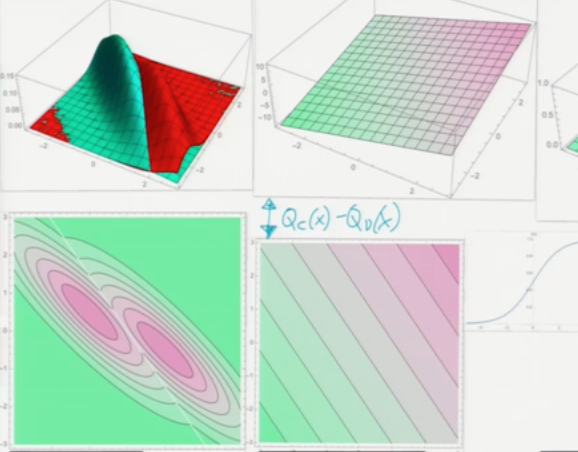
\includegraphics[scale=0.5]{images/LDA}
							\end{center}
					\end{itemize}
				\item \underline{Notes}
					\
					\begin{itemize}
						\item Changing prior $\pi_{c}$ (or loss) is easy: if its LDA adjust $\alpha$.
						\item LDA is often interpreted as projecting samples onto the normal vector.
							\begin{center}
								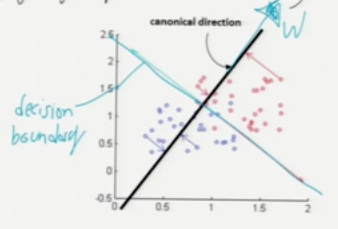
\includegraphics[scale=0.5]{images/lda_projections}
							\end{center}
						\item For 2 classes,
							\begin{itemize}
								\item LDA has $d + 1$ parameters ($w, \alpha$).
								\item QDA has $\frac{d(d+3)}{2} + 1$ parameters
								\item $\Rightarrow$ QDA more likely to overfit.
							\end{itemize}
							\begin{center}
								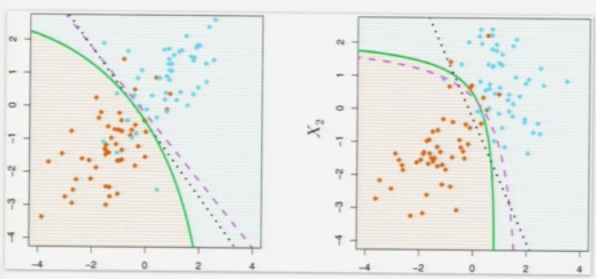
\includegraphics[scale=0.5]{images/overfitting}
							\end{center}
					\end{itemize}
			\end{itemize}


\newpage
\section*{02/24/2016}
	\subsection*{Regression} aka fitting curves to data
	\begin{itemize}
		\item Classification: given sample $x$, predict class (often binary).
		\item Regression given sample, $x$, predict a numerical value.
		\begin{itemize}
			\item Choose form of regression function $h(x;p)$ with parameters $p$.
			\begin{itemize}
				\item like predictor function in classification.
			\end{itemize}
			\item Choose a cost function (objective function) to optimize.
			\begin{itemize}
				\item Usually based on a loss function; e.g. risk function = expected loss.
			\end{itemize}
		\end{itemize}
		\item Some regression functions:
			\begin{enumerate}
				\item Linear: $h(x; w, \alpha) = w^{T}x + \alpha$.
				\item Polynomial.
				\item Logistic: $h(x; w, \alpha) = s(w^{T}x + \alpha)$. Recall: logistic function $s(\gamma) = \frac{1}{1 + e^{-\gamma}}$
			\end{enumerate}
		\item Some loss functions: let $z$ be prediction $h(x)$; $y$ be true value.
			\begin{enumerate}
				\item[A.] $L(z, y) = (z-y)^{2}$ \underline{squared error}.
				\item[B.] $L(z, y) = |z-y|$ \underline{absolute error}.
				\item[C.] $L(z, y) = -yln(z)-(1-y)ln(1-z)$ \underline{logistic loss}.
			\end{enumerate}
		\item Some cost functions to minimize:
			\begin{enumerate}
				\item[a.] $J(h) = \frac{1}{n}sum_{i=1}^{n}L(h(X_{i}),y_{i})$ \underline{mean loss}.
				\item[b.] $J(h) = \max_{i=1}^{n} L(h(X_{i}, y_{i}))$ \underline{maximum loss}.
				\item[c.] $J(h) = \sum \omega_{i}L(h(X_{i}, y_{i}))$ \underline{weighted sum}.
				\item[d.] $J(h) = \frac{1}{n}\sum L(h(X_{i}, y_{i})) + \lambda|w|^{2}$ \underline{$\ell_{2}$ penalized/regularized}.
				\item[e.] $J(h) = \frac{1}{n}\sum L(h(X_{i}, y_{i})) + \lambda|w|$ \underline{$\ell_{1}$ penalized/regularized}.
			\end{enumerate}
			\item Some combinations:
			\
			\begin{center}
				\begin{tabular}{|c|c|c|c|c|}
					\hline
					Name & Regression & Loss & Cost & Algorithm\\
					\hline
					Least-squares linear regression & 1 & A & a & quadratic, minimize w/calculus\\
					Weighted least-squares linear & 1 & A & c & quadratic, minimize w/calculus\\
					Ridge regression & 1 & A & d & quadratic, minimize w/calculus\\
					Lasso & 1 & A & d & minimize w/gradient descent\\
					Logistic regression & 3 & C & a & minimize w/gradient descent\\
					Least absolute deviations & 1 & B & a & minimize w/linear program\\
					Chebyshev criterion & 1 & B & b & minimize w/linear program\\
					\hline
				\end{tabular}
			\end{center}
	\end{itemize}
	
	\subsection*{Least-Squares Linear Regression} 1 + A + a.
	\begin{itemize}
		\item Optimization problem:
			\begin{center}
				\begin{tabular}{|c|}
					\hline
					Find $w, \alpha$ that minimizes
					$\sum_{i=1}^{n} (x_{i}\cdot w + \alpha - y_{i})^{2}$\\
					\hline
				\end{tabular}\\
				[1em]
				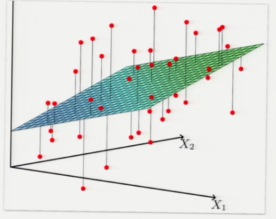
\includegraphics[scale=0.5]{images/leastsquares}
			\end{center}
		\item Convention:
			\begin{itemize}
				\item $X$ is $n$x$d$ \underline{design matrix} of samples.
				\item $y$ is $d$-vector of dependent scalars.
				\item $X = \begin{bmatrix}
					x_{11} & x_{12} & \dots & x_{1d}\\
					x_{21} & x_{22} & \dots & \\
					\vdots & \vdots & \hdots & \\
					x_{n1} & x_{n2} & \dots & x_{nd}\\
				\end{bmatrix}$
				\item Usually $n > d$.
				\item Sample row vector is $X_{i}^{T}$.
				\item Column vector is $X_{*j}$.
				\item $y = \begin{bmatrix}
						y_{0}\\
						y_{1}\\
						\vdots\\
						y_{n}
				\end{bmatrix}$
				\item Recall fictitious dimension trick: replace $x\cdot w + \alpha$ with,
					\begin{align*}
						[x_{1} \ x_{2} \ \dots \ x_{d} \ 1] \cdot \begin{bmatrix}
								w_{1}\\
								w_{2}\\
								\vdots\\
								w_{d}\\
								\alpha
							\end{bmatrix}
					\end{align*}
					Now $X$ is an $n$x($d+1$) matrix; $w$ is a ($d+1$)-vector.
				\end{itemize}
			
			\item Rewritten optimization problem:
				\begin{center}
					\begin{tabular}{|c|}
						\hline
						Find $w$ that minimizes $|Xw-y|^{2}$\\
						\hline
					\end{tabular}\\
				\end{center}
			\item Optimize by calculus, minimize residual sum of squares:
				\begin{align*}
					RSS(w) &= w^{T}X^{T}Xw - 2y^{T}Xw + y^{T}y = 0\\
						&\implies X^{T}Xw = X^{T}y \Leftarrow \text{The \underline{normal equations}}
				\end{align*}
			\item If $X^{T}X$ is singular, problem is under-constrained.
			\item We use a linear solver to find $w = (X^{T}X)^{-1}X^{T}y$.
			\item $X^{+} = (X^{T}X)^{-1}X^{T}$ is the \underline{pseudoinverse} of $X$ and is a $(d+1)$x$n$ matrix.
			\item Observe: $X^{+}X = (X^{T}X)^{-1}X^{T}X = I \Leftarrow (d+1)\text{x}(d+1)$.
			\item Observe: the predicted values of $y$ are $\hat{y} = h(x;) \Rightarrow = Xw = XX^{+}y = Hy$.
			\item where $H = XX^{+}$ is the \underline{hat matrix} because it puts the hat on $y$.
			\item Interpretation as a projection:
				\begin{itemize}
					\item $\hat{y} = Xw \in \mathbb{R}^{n}$ is a linear combination of columns of $X$.
					\item For fixed $X$, varying $w$, $Xw$ is a subspace of $\mathbb{R}^{n}$ spanned by columns.
						\begin{center}
							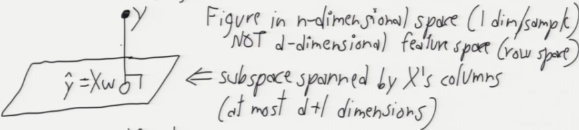
\includegraphics[scale=0.5]{images/yhat}
						\end{center}
					\item Minimizing $|\hat{y} - y|$ find point $\hat{y}$ nearest $y$ on subspace $\Rightarrow$ project $y$ onto subspace.
					\item Error is smallest when line is perpendicular to subspace: $X^{T}(Xw-y) = 0 \Rightarrow$ the normal equations!
					\item Hat matrix $H$ (also called projection matrix) does the projecting. 
				\end{itemize}
			\item Advantages:
				\begin{itemize}
					\item Easy to compute; just solve a linear system.
					\item Unique, stable solution.
				\end{itemize}
			\item Disadvantages:
				\begin{itemize}
					\item Very sensitive to outliers, because error is squared!
					\item Fails if $X^{T}X$ is singular.
				\end{itemize}
	\end{itemize}
	
	\subsection*{Logistic Regression} (David Cox, 1953) 3 + C + a
		\begin{itemize}
			\item Fits "probabilities" in range (0, 1).
			\item Usually used for classification. The input $y_{i}$'s can be probabilities, but in most applications they are all 0 or 1.
			\item QDA, LDA: generative models.
			\item Logistic regression: discriminative model.
			\item Optimization problem:
				\begin{center}
					\begin{tabular}{|c|}
					\hline
						Find $w, \alpha$ that minimizes $J = \sum_{i=1}^{n}(y_{i} \ln s(X_{i} \cdot w + \alpha) + (1-y_{i}) \ln (1 - s(X_{i} \cdot w + \alpha))$\\
						\hline
					\end{tabular}\\
					[1em]
					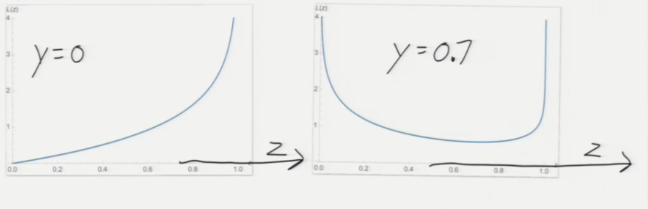
\includegraphics[scale=0.5]{images/logistics}
				\end{center}
			\item $-J(w, \alpha)$ is convex. Solve by gradient ascent.
			\begin{align*}
				s'(\gamma) &= \frac{d}{d\gamma} \frac{1}{1 + e^{-\gamma}} = \frac{e^{-\gamma}}{(1 + e^{-\gamma})^{2}}\\
				&= s(\gamma)(1 - s(\gamma))\\
			\end{align*}
			\begin{center}
				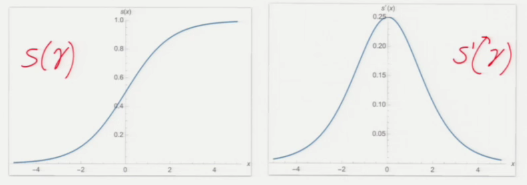
\includegraphics[scale=0.5]{images/gradients}
			\end{center}
			\item Let $s_{i} = s(X_{i}\cdot w + \alpha)$,
			\begin{align*}
				\nabla_{w} J &= \sum\Big(\frac{y_{i}}{s_{i}}\nabla s_{i} - \frac{1-y_{i}}{1 - s_{i}} \nabla s_{i}\Big)\\
					&= \sum \Big(\frac{y_{i}}{s_{i}} - \frac{1-y_{i}}{1 - s_{i}}\Big) s_{i} (1 - s_{i})X_{i}\\
					&= \sum (y_{i} - s_{i})X_{i}
			\end{align*}
			
			\item Gradient ascent rule: $w \leftarrow w + \epsilon \sum_{i=1}^{n}(y_{i} - s(X_{i}\cdot w + \alpha))X_{i}$
			\item Stochastic gradient ascent: $w \leftarrow w + \epsilon(y_{i} - s(X_{i}\cdot w + \alpha))X_{i}$ works best if we shuffle samples in random order; process one by one.
			\item For very large $n$, sometimes converges before we visit all samples!
			\item Starting from $w=0, \alpha=0$ works well in practice.
			\begin{center}
				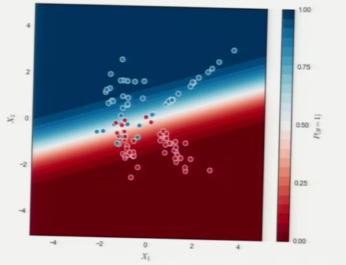
\includegraphics[scale=0.5]{images/regression}
			\end{center}
		\end{itemize}


\newpage
\section*{02/29/2016}
	\subsection*{Weighted Least-Squares Regression}
	\
	\begin{itemize}
		\item Assign each sample a weight $\omega_{i}$; collect them in an $n$x$n$ diagonal matrix $\Omega$.
		\item Greater $\omega_{i} \Rightarrow$ work harder to minimize $|\hat{y_{i}} - y_{i}|$. Recall: $\hat{y} = Xw$.
		\item Optimization problem:
			\begin{center}
				\begin{tabular}{|c|}
					\hline
					Find $w$ that minimizes $(Xw - y)^{T} \Omega (Xw-y)$\\
					\hline
				\end{tabular}\\
			\end{center}
		\item Note,
			\begin{align*}
				(Xw - y)^{T}\Omega (Xw-y) = \sum_{i=1}^{n} \omega_{i}((Xw)_{i} - y_{i})^{2}\\
			\end{align*}
		\item Sove for $w$ in normal equations:	
			\begin{align*}
				X^{T}\Omega Xw = X^{T}\Omega y
			\end{align*}
		\item Note: $\Omega^{\frac{1}{2}}\hat{y}$ is orthogonal projections of $\Omega^{\frac{1}{2}}y$ onto subspace spanned by columns of $\Omega^{\frac{1}{2}}X$.
	\end{itemize}
	
	\subsection*{Newton's Method}
	\
		\begin{itemize}
			\item Iterative optimization method for smooth functions $J(w)$ often much faster than gradient descent.
			\item Idea: You're at point $v$ in a space, where you're trying to optimize $w$. Approximate $J(w)$ near $v$ by quadratic function. Jump to its unique critical point. Repeat until bored.
			\item Taylor series about $v$:
				\begin{align*}
					\nabla J(w) = \nabla J(v) + (\nabla^{2}J(v))(w-v) + \mathcal{O}(|w - v|^{2})
				\end{align*}
			\item $\nabla^{2}J(v)(w-v)$ is the \underline{Hessian matrix} of $J$ at $v$.
			\item Find critical point $w$ by setting $\nabla J(w) = 0$:
				\begin{align*}
					w = v - (\nabla^{2}J(v))^{-1}\nabla J(v)
				\end{align*}
			\end{itemize}
\begin{codeblock}
	Newton's Method:
	    while not "converged":
	        $e \leftarrow$ solution to linear system $(\nabla^{2}J(w))e = -\nabla J(w)$
	        $w \leftarrow w + e$
\end{codeblock}
			\begin{itemize}
			\item Warning: Doesn't know difference between min, max or saddle points. Starting point must be "close enough" to desired solution.
			\item Facts:
				\begin{itemize}
					\item If objective function $J$ is actually a quadratic function, you'll jump to the minimum in one iteration. The closer $J$ is to quadratic the faster it is, and vice versa.
					\item Superior to blind gradient descent: 1) Doesn't just take a blind step length downhill it actually tries to figure out the bottom of the curve. 2) It doesn't just pick one direction of steepest descent it tries to optimize all at once.
					\item Biggest disadvantage: Computing the Hessian is very expensive. 
				\end{itemize}
		\end{itemize}
		
		\subsection*{Logistic Regression}
			\
			\begin{itemize}
				\item Recall: $s'(\gamma) = s(\gamma)(1 - s(\gamma))$, $s_{i} = s(X_{i}\cdot w)$.
				\item $\nabla_{w}J(w) = \sum_{i=1}^{n}(y_{i} - s_{i})X_{i} = X^{T}(y - s)$, where $s$ is n-vector with components $s_{i}$.
					\begin{align*}
						\nabla^{2}J(w) = -\sum_{i=1}^{n}s_{i}(1 - s_{i})X_{i}X_{i}^{T} = X^{T}\Omega X
					\end{align*}
				where $\Omega$ is a diagonal matrix with components $s_{i}(1 - s_{i})$.
				\item $\Omega$ is positive definite for all $w$,so $X^{T}\Omega X$ is positive semidefinite, so $-J(w)$ is convex.
				\end{itemize}
\begin{codeblock}
	Newton's Method:
	    while not "converged":
	        Solve for $e$ in normal equations: $(X^{T}\Omega X)e = X^{T}(y - s)$
	        $w \leftarrow w + e$
\end{codeblock}
				Remember $\Omega, s$ are functions of $w$.
				\begin{itemize}
				\item An example of "iteratively re-weighted least squares."
				\item $\Omega$ prioritizes samples with $s_{i}$ near 0.5; tunes out samples that are near 0/1.
				\item Idea: If n very large, save time by using a random subsample of the samples per iteration. Increase sample size as you go.
			\end{itemize}
			
		\subsection*{LDA vs. Logistic regression}
		\
				\begin{itemize}
					\item Advantages of LDA:
						\begin{itemize}
							\item For well-separated classes, LDA stable; logistic regression surprisingly unstable.
							\item For more than 2 classes easy \& elegant, logistic regression needs modifying ("softmax regression").
							\item Slightly more accurate when classes nearly normal, especially if n is small.
						\end{itemize}
					\item Advantages of Logistic regression:
						\begin{itemize}
							\item More emphasis on decision boundary.
							\begin{center}
								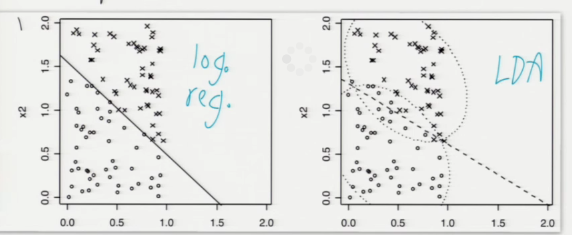
\includegraphics[scale=0.5]{images/ldavsregression}
							\end{center}
							\item Hence less sensitive to outliers.
							\item Easy and elegant treatment of "partial" class membership; LDA is all-or-nothing.
							\item More robust on some non-gaussian distributions (e.g. large skew).
						\end{itemize}
					\item ROC Curve
						\begin{center}
							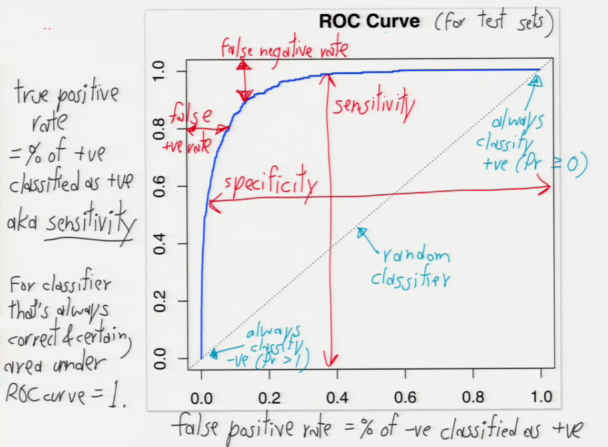
\includegraphics[scale=0.5]{images/ROCCurve}
						\end{center}
						\begin{itemize}
							\item Receiver Operating Characteristics 
							\item A way of telling you information about the test set, not part of the learning algorithm.
							\item Run classifier on test set, and it shows the rate of false positives vs. true positives for a range of settings.
							\item x-axis false positive rate = \% of negative samples accidentally classified as positive.
							\item y-axis true positive rate = \% of positive that actually got classified as positive (aka sensitivity).
						\end{itemize}
				\end{itemize}
				
		\subsection*{Least-Squares Polynomial Regression}
				\
					\begin{itemize}
						\item Replace each $X_{i}$ with feature vector $\Phi(X_{i})$ with all terms of degree $0 \dots p$.
						\item e.g. $\phi(X_{i}) = \begin{bmatrix}
												X_{i1}^{2} & X_{i1}X_{i2} & X_{i2}^{2} & X_{i1} & X_{i2} & 1 
 											\end{bmatrix}^{T}
 											$
 						\item Can also use non-polynomial features (e.g. edge detectors).
 						\item Otherwise just like linear or logistic regression.
 						\item Logistic regression plus quadratic features = same logistic posteriors as QDA. Very easy to overfit!
							\begin{center}
								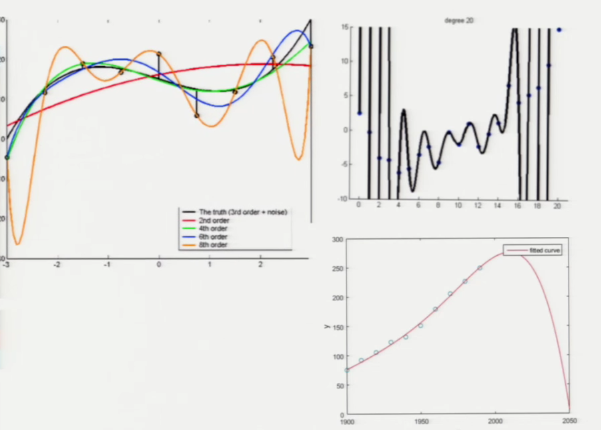
\includegraphics[scale=0.5]{images/polyregression}
							\end{center}
					\end{itemize}

\newpage
\section*{03/02/2016}
	\subsection*{Statistical Justification for Regression}
	\
	\begin{itemize}
		\item Typical model of reality:
			\begin{itemize}
				\item Samples come from unknown probability distribution $X_{i} \sim D$.
				\item y-values are sum of unknowns, non-random surface plus random noise: for all $X_{i}$,
					\begin{align*}
						y_{i} = f(X_{i}) + \epsilon_{i}
					\end{align*}
			\end{itemize}
		\item Goal of regression: find $h$ that estimates f.
		\item Ideal approach: choose $h(x) = E_{y}[Y | X=x]$
	\end{itemize} 
	
	\subsection*{Least-squares Regression from Max Likelihood}
	\
	\begin{itemize}
		\item Suppose $\epsilon_{i} \sim \mathcal{N}(0, \sigma^{2})$; then $y_{i}|X_{i} \sim \mathcal{N}(f(X_{i}), \sigma^{2})$.
		\item Recall that log likelihood for normal distribution is,
			\begin{align*}
				ln P(y_{i}) &= - \frac{|y_{i} - \mu|^{2}}{2\sigma^{2}} - constant \ \ \ \ \ \ \Leftarrow \mu = f(X_{i})\\
				ln(P(y_{1})P(y_{2}) \dots P(y_{n})) &= ln P(y_{1}) + ln P(y_{2}) + \dots + ln P(y_{n})\\
			\end{align*}
		\item Takeaway: If you apply the principle of max likelihood to linear regression with an input model that assumes gaussian noise $\Rightarrow$ find $f$ by least-squares. 
	\end{itemize}
	
	\subsection*{Empirical Risk}
	\
	\begin{itemize}
		\item The \underline{risk} for hypothesis $h$ is the expected loss $R(h) = E[L]$ over all $X, Y$.
		\item Discriminative model: we don't know $X'$s distribution D. How can we minimize the risk?
		\item \underline{Empirical distribution}: A discrete probability that is the sample set, with each sample equally likely.
		\item \underline{Empirical risk}: expected loss over empirical distribution $\hat{R}(h) = \frac{1}{n} \sum_{i=1}^{n} L(h(X_{i}), y_{i}))$.
		\item Takeaway: this is why we minimize the sum of loss functions.
	\end{itemize}
	
	\subsection*{Logistic regression from Max Likelihood}
	\
	\begin{itemize}
		\item If we accept the logistic regression function, what cost function should we use?
		\item Given arbitrary sample $x$, write probability it is in (not in) the class: (fictitious dimension: x ends w/1; $w$ ends w/$\alpha$).
			\begin{align*}
				P(y=1|x;w) &= h(x;w) \ \ \ \ \ \ \ \ \Leftarrow h(x;w) = s(w^{T}x)\\
				P(y=0|x;w) &= 1 - h(x;w)\\
			\end{align*}
		\item Combine these 2 facts into 1 expression:
			\begin{align*}
				P(y|x;w) = h(x)^{y}(1 - h(x))^{1-y}\\
			\end{align*}
		
		\item Likelihood is,
			\begin{align*}
				L(w; x_{1}, \dots, x_{n}) &= \prod_{i=1}^{n} P(y_{i}|X_{i};w)\\
				l(w) = ln L(w) &= \sum_{i=1}^{n} ln P(y_{i}|X_{i};w)\\
				&= \sum (y_{i}ln h(X_{i}) + (1-y_{i})ln(1-h(X_{i})))
			\end{align*}
		\item which is negated logistic cost function J(w).
	\end{itemize}
	
	\subsection*{The Bias-variance Decomposition}
	\
	\begin{itemize}
		\item There are 2 sources of error in a hypothesis h:
			\begin{itemize}
				\item \underline{bias}: error due to inability of hypothesis $h$ to fit $f$ perfectly. e.g. fitting quadratic $f$ with a linear $\ell$.
				\item \underline{variance}: error due to fitting random noise in data. e.g. we fit linear $f$ with a linear $h$, yes $h \neq f$.
			\end{itemize}
		\item Model: generate samples $X_{1} \dots X_{n}$ from some distribution $D$. Values $y_{i} = f(X_{i}) + \epsilon_{i}$. Fit hypothesis $h$ to $X, y$.
		\item Now $h$ is a random variable; i.e. its weights are random.
		\item Consider an arbitrary point $z \in \mathbb{R}^{d}$ (not necessarily a sample!) and $\gamma = f(z) + \epsilon$.
		\item Note: $\text{E}[\gamma] = f(z) ; \text{Var}(\gamma) = \text{Var}(\epsilon)$;
		\item Risk function when loss is squared error:
		\item Here we are taking the expectation over all possible training sets $X,y$ and values of $\gamma$.
			\begin{align*}
				R(h) &= E[L(h(z), \gamma)]\\
					&= E[(h(z) - \gamma)^{2}]\\
					&= E[h(z)^{2}] + E[\gamma^{2}] - 2E[\gamma h(z)]\\
					&= \text{Var}(h(z)) + E[h(z)]^{2} + \text{Var}(\gamma) + E[\gamma]^{2} - 2E[\gamma]E[h(z)]\\
					&= (E[h(z)] - E[\gamma])^{2} + \text{Var}(h(z)) + \text{Var}(\gamma)\\
					&= E[h(z) - f(z)]^{2} + \text{Var}(h(z)) + \text{Var}(\epsilon)\\
			\end{align*}
			\begin{itemize}
				\item We take expectation over possible training sets, $X, y$ and values of $\gamma$.
				\item $E[h(z) - f(z)]^{2}$: is square of the bias of method.
				\item $\text{Var}(h(z))$: variance of method.
				\item $\text{Var}(\epsilon)$: irreducible error (comes from test point not from training).
			\end{itemize}
			
			\item This is point-wise version. Mean version: Let $z \sim D$ be random variable; take expectation of the squares bias, variance over $z$
				\begin{center}
					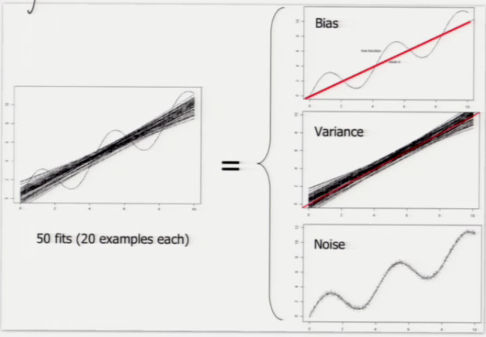
\includegraphics[scale=0.5]{images/noise}
				\end{center}
				\begin{itemize}
					\item Under-fitting: too much bias.
					\item Over-fitting caused by too much variance. 
				\end{itemize}
			\item Training error reflects bias but not variance; test error reflects both.
			\item For many distributions, variance $\rightarrow$ 0 as $n \rightarrow \infty$.
			\item If $h$ can fit $f$ exactly, for many distributions bias $\rightarrow 0$ as $n \rightarrow \infty$.
			\item If $h$ cannot fit $f$ well, bias is large at "most" points.
			\item Adding a good feature reduces bias; adding a bad feature rarely increases it.
			\item Adding a feature usually increases variance.
			\item Cannot reduce irreducible error.
			\item Noise in test set affects only var($\epsilon$); noise in training set affects only bias and Var(h).
			\item For real-world data, $f$ is rarely knowable (and noise model might be wrong).
			\item But we can test learning algorithms by choosing $f$ and making synthetic data.
				\begin{center}
					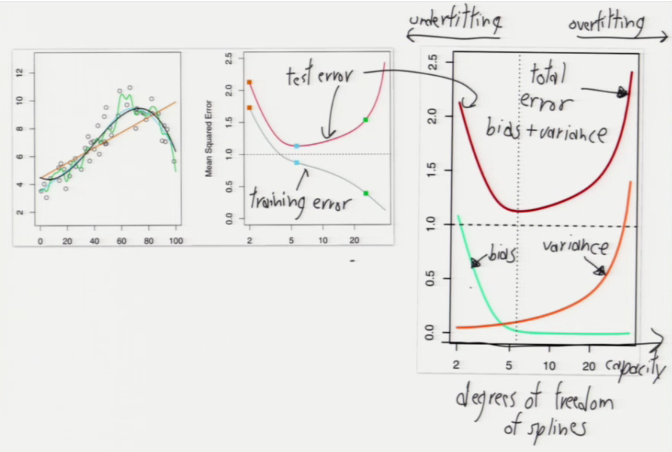
\includegraphics[scale=0.5]{images/errorvsbias}
				\end{center}
			\item Example: Least-Squares Linear Regression:
				\begin{itemize}
					\item No fictitious dimension.
					\item Model: $f(z) = v^{T}z$.
					\item Let $e$ be a noise n-vector $e\sim \mathcal{N}(0, \sigma^{2})$.
					\item Training values: $y = Xv + e$. Input to regression algorithm are $y, X$.
					\item Linear regression computes weights:
						\begin{align*}
							w = X^{+}y = X^{+}(Xv + e) = v + X^{+}e
						\end{align*}
					\item Bias is,
						\begin{align*}
							E[h(z) - f(z)] = E[w^{T}z - v^{T}z] = E[z^{T}X^{+}e] = z^{T}X^{+}E[e] = 0
						\end{align*}
					\item Warning: This does not mean $h(z) - f(z)$ is everywhere 0. Sometimes positive, sometimes negative, mean over training sets is 0.
					\item Variance is,
						\begin{align*}
							\text{Var}(h(z)) &= \text{Var}(w^{T}z) = \text{Var}(z^{T}w)\\ 
							&= \text{Var}(z^{T}(v + X^{+}e)\\
							&= \text{Var}(z^{T}v + z^{T}X^{+}e))\\ 
							&= \text{Var}(z^{T}X^{+}e)\\
							&= \sigma^{2} |z^{T}X^{+}|^{2}\\
							&= \sigma^{2} |z^{T}(X^{T}X)^{-1}X^{T})|^{2}\\
							&= \sigma^{2} z^{T}(X^{T}X)^{-1}X^{T}X(X^{T}X)^{-1}z\\
							&= \sigma^{2}z^{T}(X^{+}X)^{-1}z
						\end{align*}
					\item If choose coordinate system so $E[X] = 0$ it simplifies to $\approx \sigma^{2}\frac{d}{n}$.
					\item Takeaways: Bias can be zero when hypothesis function can fit the real one. Variance portion of RSS (overfitting) decreases as $\frac{1}{n}$, increases as $d$.
				\end{itemize}
	\end{itemize}

\newpage
\section*{03/07/2016}
	\subsection*{Ridge Regression} (aka Tikhonov regularization)
	\
	\begin{itemize}
		\item (1) + (A) + $\ell_{2}$ penalized mean loss (d).
		\item Optimization problem $J(w)$:
		\begin{center}
			\begin{tabular}{|c|}
				\hline
				Find $w$ that minimizes
				$|Xw - y|^{2} + \lambda||w'||^{2}$\\
				\hline
			\end{tabular}\\
		\end{center}
		Where $w'$ is $w$ with components $\alpha$ replaced by 0. $X$ has fictitious dimension but we DON'T penalize $\alpha$.
		\item Adds a penalty term to encourage small $|w'|$ -- called \underline{shrinkage}.
		\item Why? Guaranteed positive definite normal equations; always unique solution. e.g. when $d>n$ always semi-definite.
			\begin{center}
				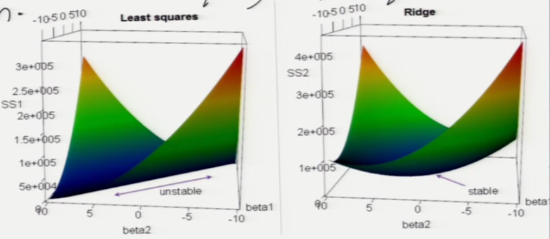
\includegraphics[scale=0.5]{images/ridge}
			\end{center}
		\item Reduces over-fitting by reducing variance by penalizing large weights.
			\begin{center}
				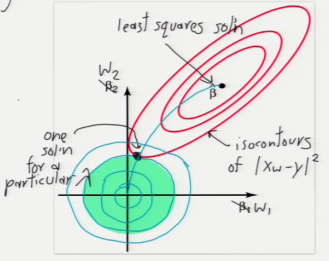
\includegraphics[scale=0.5]{images/sqrsvslambda}
			\end{center}
		\item Setting $\nabla J = 0$ gives equations,
			\begin{align*}
				(X^{T}X + \lambda I')w = X^{T}y
			\end{align*} 
		\item where $I'$ is identity matrix with bottom right set to zero.
		\item Algorithm: solve for $w$. Return $h(z) = w^{T}x$.
		\item Increasing $\lambda \Rightarrow$ more \underline{regularization}; smaller $|w'|$.
		\item Given our data model $y = Xv + e$, where $e$ is noise.
		\item Variance of ridge regression is Var($x^{T}(X^{T}X + \lambda I')^{-1}X^{T}e)$.
		\item As $\lambda \rightarrow \infty$, variance $\rightarrow 0$, but bias increases.
			\begin{center}
				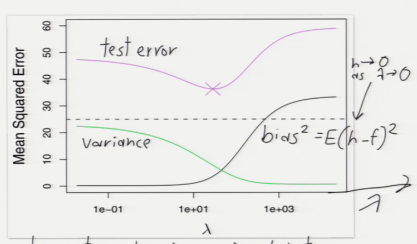
\includegraphics[scale=0.5]{images/lambdabiasvsvariance}
			\end{center}
		\item $\lambda$ is a hyper-parameter; tune by (cross)-validation.
		\item Ideally features should be "normalized" to have same variance.
		\item Alternative: Use asymmetric penalty by replacing $I'$ with other diagonal matrix.
	\end{itemize} 
	
	\subsection*{Bayesian justification for ridge regression}
	\
	\begin{itemize}
		\item Assign a prior probability on $w'$: a Gaussian centered at 0.
		\item Posterior probability $\approx$ likelihood of $w \cdot $ prior $P(w') \leftarrow$ Gaussian PDF. 
		\item Maximize the log posterior, $\ell$n likelihood + $\ell n P(w') =$ -const$|Xw-y|^{2}$ - const$|w'|^{2}$ - constant.
		\item This method (using likelihood, but maximizing posterior) is called \underline{maximum a posteriori} (MAP).
	\end{itemize}
	
	\subsection*{Kernels}
	\
	\begin{itemize}
		\item Recall: with $d$ input features, degree-p polynomials blow up to $\mathcal{O}(d^{p})$ features.
		\item Today we use magic to use those features without computing them!
		\item Observation: In many learning algorithms:
			\begin{itemize}
				\item The weights can be written as a linear combination of input samples.
				\item We can use inner products of $\phi(x)'$s only $\Rightarrow$ don't need to compute $\phi(x)$!
				\item Suppose $w = X^{T}a = \sum_{i=1}^{n} a_{i}X_{i}$ for some $a \in \mathbb{R}^{n}$.
				\item Substitute this identity into algorithms and optimize $n$ \underline{dual weights} (aka \underline{dual parameters} a, instead of $d+1$ \underline{primal weights} w.
			\end{itemize}
	\end{itemize}
	
	\subsection*{Kernel Ridge Regression}
	\
	\begin{itemize}
		\item \underline{Center} $X$ and $y$ so their means are zero; $X_{i} \leftarrow X_{i} - \mu_{x}$. By centering the matrix we minimize the penalization of $\alpha$
		\item This lets us replace $I'$ with $I$ in normal equations:
			\begin{align*}
				&(X^{T}X + \lambda I)w = X^{T}y\\
				&\Rightarrow w = \frac{1}{\lambda}(X^{T}y - X^{T}Xw) = X^{T}a  \ \ \ \ \ \text{where } a = \frac{1}{\lambda}(y-Xw)
			\end{align*}
		\item This shows that $w$ is a linear combination of samples. To compute $a$:
			\begin{align*}
				\lambda a = (y - XX^{T}a) \Rightarrow a = (XX^{T} + \lambda I)^{-1}y
			\end{align*}
		\item $a$ is the \underline{dual solution}; solves the \underline{dual form} of ridge regression:
		\begin{center}
			\begin{tabular}{|c|}
				\hline
				Find $a$ that minimizes $|XX^{T} - y|^{2} + \lambda|X^{T}a|^{2}$\\
				\hline
			\end{tabular}\\
		\end{center}
		\item Regression function is:
			\begin{align*}
				h(z) = w^{T}z = a^{T}Xz = \sum_{i=1}^{n} a_{i}(X_{i}^{T}z) \Leftarrow \text{weighted sum of inner products}
			\end{align*}
		\item Let $k(x, z) = x^{T}z$ be \underline{kernel function}.
		\item Let $K = XX^{T}$ be nxn \underline{kernel matrix}. Note $K_{ij} = k(X_{i}, X_{j})$.
		\item $K$ is singular if $n>d$. In that case no solution if $\lambda = 0$.
		\item Summary of kernel ridge regression:
			\begin{itemize}
				\item Solve $(K + \lambda I)a = y$  for a $\Leftarrow \mathcal{O}(n^{3})$ time.
				\item $K_{ij} = k(X_{i}, X_{j}) \ \forall i,j \Leftarrow \mathcal{O}(n^{2}d)$ time.
				\item for each test point $z$: $h(z) = \sum_{i=1}^{n} a_{i} k(X_{i}, z) \Leftarrow \mathcal{O}(nd)$ time.
			\end{itemize}
		\item Do not use $X$ directly: only $k(\cdot , \cdot)$.
		\item Dual: solve $n$x$n$ linear system.
		\item Primal: solve $d$x$d$ linear system.
	\end{itemize}
	
	\subsection*{The Kernel Trick} (aka \underline{kernelization})
	\
	\begin{itemize}
		\item The \underline{polynomial kernel} of degree $p$ is $k(x,z) = (x^{T}z + 1)^{p}$.
		\item Theorem: $(x^{T}z + 1)^{p} = \phi(x)^{T}\phi(z)$ where $\phi(x)$ contains every monomial in $x$ of degree $0 \dots p$.
		\item Example for $d=2, p=2$.
			\begin{align*}
				(x^{T}z+1)^{2} &= x_{1}^{2}z_{1}^{2} + x_{2}^{2}z_{2}^{2} + 2x_{1}z_{1}x_{2}z_{2} + 2x_{1}z_{1} + 2x_{2}z_{2} + 1\\
					& = \begin{bmatrix}
						x_{1}^{2} & x_{2}^{2} & \sqrt{2x_{1}x_{2}} & \sqrt{2x_{1}} & \sqrt{2x_{2}} & 1
					\end{bmatrix}
					\cdot
					\begin{bmatrix}
						z_{1}^{2}\\
						z_{2}^{2}\\
						\sqrt{2z_{1}z_{2}}\\
						\sqrt{2z_{1}}\\
						\sqrt{2z_{2}}\\
						1\\
					\end{bmatrix}\\
					&= \phi(x)^{T} \phi(z)\\
			\end{align*}
		\item Key win: compute $\phi(x)^{T} \phi(z)$ in $\mathcal{O}(d)$ time instead of $\mathcal{O}(d^{p})$ even though $\phi(x)$ has length $\mathcal{O}(d^{p})$.
		\item Kernel ridge regression replaces $X_{i}$ with $\phi(X_{i})$:
			\begin{itemize}
				\item Let $k(x, z) = \phi(x)^{T}\phi(z)$.	
			\end{itemize} 
	\end{itemize}


\newpage
\section*{03/09/2016}
	\subsection*{Kernels} continued
	\begin{itemize}
		\item \underline{Kernel Perceptrons}
		\item Note: Everywhere below, we can replace $X_{i}$ with $\phi(X_{i})$
		\end{itemize}

\begin{codeblock}
	Perceptron Algorithm:
	    while (some $y_{i}X_{i} \cdot w < 0$):
	        $w \leftarrow w + \epsilon y_{i}x_{i}$
	    while (still have test points $z$):
	        $f(z) \leftarrow w^{T}x$
\end{codeblock}
		\begin{itemize}
		\item Kernelize with $w=X^{T}a$; $X_{i}\cdot w = (XX^{T}a)_{i} = (Ka)_{i}$.
		\end{itemize}

\begin{codeblock}
	Dual Perceptron Algorithm:
	    $a = [y_{1}, 0, \dots, 0]^{T}$
	    $K_{ij} = K(X_{i}, X_{j}) \ \forall i,j$
	    while (some $y_{i}(Ka)_{i} \cdot w < 0$):
	        $a \leftarrow a + \epsilon y_{i}$
	    while (still have test points $z$):
	        $f(z) \leftarrow \sum_{j=1}^{n} a_{j}K(X_{j},z)$
\end{codeblock}
		\begin{itemize}
		\item Computing $K_{ij} \Leftarrow \mathcal{O}(n^{2}d)$ time (kernel trick).
		\item Optimization for first while loop: maintain $Ka$, $\mathcal{O}(n)$ time.
		\item Second loop runs in $\mathcal{O}(nd)$ time or we can compute $w=X^{T}a$ once in $\mathcal{O}(nd')$ time and evaluate test points in $\mathcal{O}(d')$ time per point, where $d'$ is the length of $\phi(\cdot)$.
	\end{itemize}

	\subsection*{Kernel Logistic Regression}
	\
	\begin{itemize}
		\item Stochastic gradient ascent step:
			\begin{align*}
				a_{i} \leftarrow a_{i} + \epsilon(y_{i} - s((Ka)_{i}))\\
			\end{align*}
		\item Gradient ascent step:
			\begin{align*}
				a \leftarrow a + \epsilon(y_{i} - s((Ka)) \Leftarrow \text{ applying s component-wise to vector } Ka \\
			\end{align*}	
		\item for each test point $z$: $h(z) \leftarrow s(\sum_{j=1}^{n} a_{j}k(X_{j}, z))$.
	\end{itemize}
	
	\subsection*{The Gaussian Kernel}
	\
	\begin{itemize}
		\item \underline{Gaussian kernel}, aka \underline{radial basis function kernel}
		\item There exists a $\phi(x)$ such that:
			\begin{align*}
				k(x, z) = e^{(-\frac{|x-z|^{2}}{2\sigma^{2}})}
			\end{align*}
		\item Key observation: $h(z) = s(\sum_{j=1}^{n} a_{j}k(X_{j}, z))$ is a linear combination of Gaussian centered at samples.
		\item Very popular in practice:
			\begin{itemize}
				\item Gives very smooth $h$
				\item Behaves somewhat like k-nearest neighbor, but smoother.
				\item Oscillates less than polynomial (depending on $\sigma$).
				\item $k(x,z)$ can be interpreted as a "similarity measure" $y$ value more influenced by points around it.
				\item Gaussian is maximum when $x=z$, goes to 0 as distance increases.
				\item Samples "vote" for value at $z$, but closer samples get bigger vote.
			\end{itemize}
		\item $\sigma$ trades off bias vs. variance:
			\begin{itemize}
				\item larger $\sigma \rightarrow$ wider Gaussians, smoother $h \rightarrow$ more bias, less variance.
				\item Choose by (cross)-validation.
			\end{itemize}
	\end{itemize}
	
	\subsection*{Subset Selection}
	\begin{itemize}
		\item All features increase variance, but not all features reduce bias.
		\item Idea: Identify poorly predictive features, ignore them (weight zero). Less over-fitting, lower test errors.
		\item 2nd motivation: Inference. Simpler models convey interpretable wisdom. Useful in all classification and regression methods. Sometimes it's hard: Different feature can partly encode some info. Combinatorially hard to choose best feature subset.
		\item Algorithm: Best subset selection. Try all $2^{d} - 1$ nonempty subsets of features. Choose the best model by cross-validation. This is very slow!
		\item Heuristic: \underline{Forward stepwise selection}.
		\begin{itemize}
			\item Start with \underline{null model} (0 features); repeatedly add best feature. Repeat until test errors start increasing (due to over-fitting).
			\item Requires training $\mathcal{O}(d^{2})$ models instead of $\mathcal{O}(2^{d})$.
			\item Not perfect.
		\end{itemize}
		\item Heuristic: \underline{Backward stepwise selection}.
		\begin{itemize}
			\item Start with all $d$ features; repeatedly remove feature whose removal gives best reduction in test error.
			\item Also trains $\mathcal{O}(d^{2})$ models.
		\end{itemize}
		\item If you think there's only a few good features do forward, if you think most features will be good do backwards.
	\end{itemize}
	
	\subsection*{Lasso (Tibsharani, 1996)}
	\begin{itemize}
		\item Regression with regularization: (1) + (A) + $\ell_{1}$ penalized mean loss (e) "Least absolute shrinkage and selection operator"
		\item Optimization problem:
		\begin{center}
			\begin{tabular}{|c|}
				\hline
				Find $w$ that minimizes $|Xw-y|^{2} + \lambda|w'|_{1}$\\
				\hline
			\end{tabular}\\
		\end{center}
		where $|w'|_{1} = \sum_{i=1}^{n}|w_{i}|$.
		\item Recall ridge regression: isosurfaces of $|w'|_{2}^{2}$ are hyperspheres. 
		\item The isosurfaces of $|w'|_{1}$ are \underline{cross-polytopes}.
		\item The unit cross-polytope is the convex hull of all the positive and negative unit coordinate vectors.
		\begin{center}
			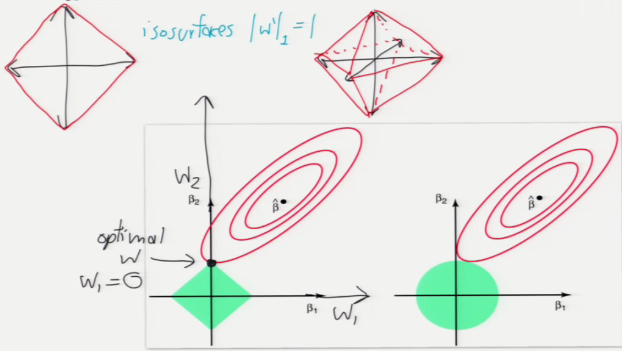
\includegraphics[scale=0.6]{images/lassol1}
			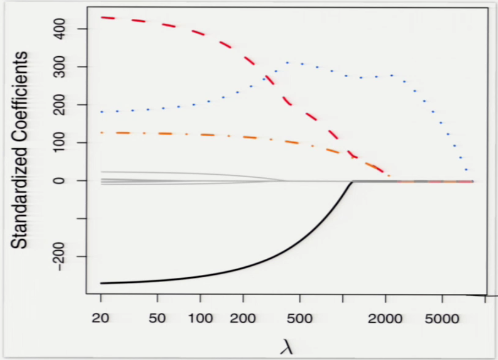
\includegraphics[scale=0.6]{images/standarizesweights}
		\end{center}
		
		\item Algorithms to optimize: subgradient descent, least-angle regression (LARS), forward stagewise.
	\end{itemize}
	
\newpage
\section*{03/14/2016}
\subsection*{Decision Trees}
	\begin{itemize}
		\item Non-linear method for classification.
		\item Uses trees with two node types:
			\begin{itemize}
				\item internal nodes test feature values (usually just one) and branch accordingly.
				\item leaf nodes specify class $h(x)$.	
				\begin{center}
					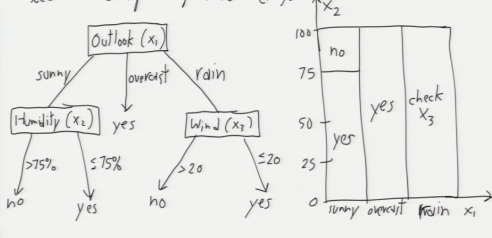
\includegraphics[scale=0.6]{images/tree:graph}
				\end{center}
			\end{itemize}
		\item Cuts x-space into rectangular cells.
		\item Works well with both categorical and quantitative features.
		\item Interpretable result (inference).
		\item Decision boundary can be arbitrarily complicated.
			\begin{itemize}
				\item Can really reduce bias if boundary is truly complicated.
				\item A lot of opportunity for over-fitting.
				\begin{center}
					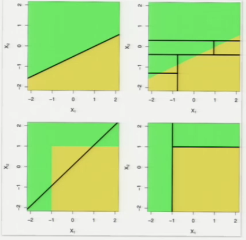
\includegraphics[scale=0.8]{images/decisiontreeexamples}
				\end{center}
			\end{itemize}
		\item Leaf is pure if every training sample in it has the same class.
		\item Consider classification first: Greedy, top-down learning heuristic: 
		\item Let $S \subseteq \{1, 2, \dots, n\}$ be a list of sample indices.
		\item Top level call: $S = \{1, 2, \dots, n\}$
		\end{itemize}
\begin{codeblock}
	GrowTree($S$):
	    if ($y_{i} = c \ \forall i \in S$ and some class C):
	        return new leaf(C)
	    else:
	        choose best splitting feature $j$ and splitting point $\beta$ (*)
	        $S_{\ell} = \{i : X_{ij} < \beta \}$
	        $S_{r} = \{ : X_{ij} \geq \beta \}$
	        return new node($j, \beta, $GrowTree$(S_{\ell}), $GrowTree$(S_{r}))$
\end{codeblock}
	\begin{itemize}
		\item (*) How to choose best split?
			\begin{itemize}
				\item Try all splits.
				\item For a set $S$, let $J(S)$ be the \underline{cost} of $S$.
				\item Choose the split that minimizes $J(S_{\ell}) + J(S_{r})$; or, the split that minimizes the weighted average $\frac{|S_{\ell}|J(S_{\ell})+ |S_{r}|J(S_{r})}{|S_{\ell}| + |S_{r}|}$
			\end{itemize}
		\item How to choose cost $J(S)$?
			\begin{itemize}
				\item Idea 1 (bad): Label $S$ with the class $C$ that labels the most samples in $S$. $J(S) \leftarrow$ number of samples in $S$ not in class $C$.
				\begin{center}
					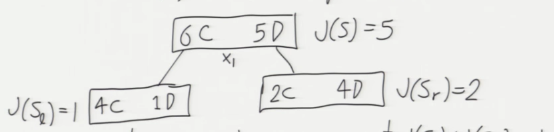
\includegraphics[scale=0.6]{images/idea1good}
				\end{center}
				\begin{itemize}
					\item Problem: sometimes we make "progress," yet $J(S_{\ell}) + J(S_{r}) = J(S)$.
				\begin{center}
					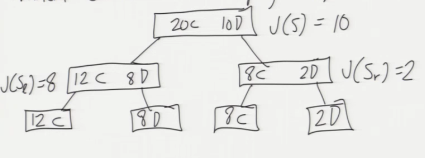
\includegraphics[scale=0.6]{images/idea1bad}
				\end{center}
				\end{itemize}
				\item Idea 2 (good): Measure \underline{entropy}.
				\begin{itemize}
					\item Let $Y$ be a random class variable, and suppose $P(Y=C) = p_{c}$.
					\item The \underline{surprise} of $Y$ being class $C$ is $S(Y=C) = -log_{2} \ p_{c}$.
						\begin{itemize}
							\item event with probability 1 gives us zero surprise.
							\item event with probability 0 gives us infinite surprise.
						\end{itemize}
					\item The \underline{entropy} of an index set $S$ is the average surprise: $H(S) = -\sum_{c} p_{c} \ log_{2} \ p_{c}$, where $p_{c} = \frac{|\{i \in S : y_{i} = C\}|}{|S|}$
					\item If all samples in $S$ belong to same class? $H(S) = -1 \ log_{2} \ 1 = 0$.
					\item Half class $C$, half class $D$? $H(S) = -\frac{1}{2} \ log_{2} \frac{1}{2} - \frac{1}{2} \ log_{2} \frac{1}{2} = 1$.
					\item n samples, all different classes? $H(S) = -log_{2} \ \frac{1}{n} = log_{2} \ n$.
					\begin{center}
						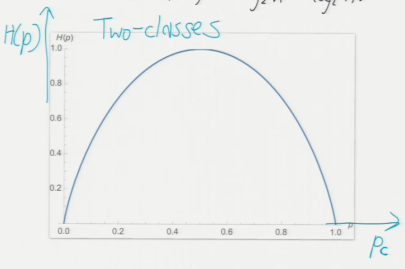
\includegraphics[scale=0.7]{images/entropy}
					\end{center}
				\end{itemize}
				
			\item Weighted average entropy after split is $H_{after} = \frac{|S_{\ell}|H(S_{\ell})+ |S_{r}|H(S_{r})}{|S_{\ell}| + |S_{r}|}$
			\item Choose split that maximizes \underline{information gain} $H(S) - H_{after}$.
			\begin{center}
				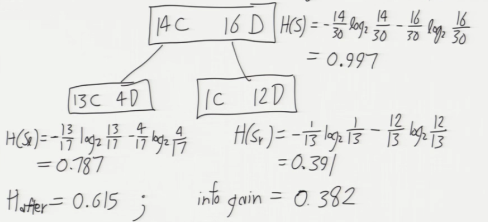
\includegraphics[scale=0.6]{images/informationgain}
			\end{center}
			\item Information gain always positive expect when one child is empty or \\ $\ \forall C, P(y_{i} = C|i \in S_{\ell}) = P(y_{i}=C|i \in S_{r})$ 
			\begin{center}
				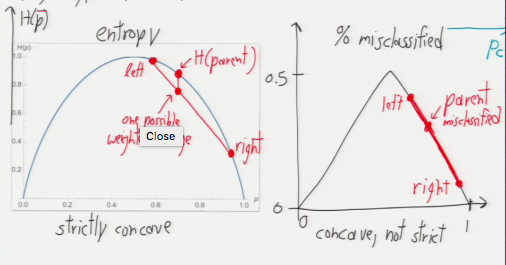
\includegraphics[scale=0.7]{images/idea1vsidea2}
			\end{center}
			\end{itemize}
		\item More on choosing a split.
			\begin{itemize}
				\item For binary feature $x_{i}$, children are $x_{i}=0$ and $x_{i}  =1$.
				\item If $x_{i}$ has 3+ discrete values, split depends on application.
				\item If $x_{i}$ is quantitative, sort samples in $S$ by feature $x_{i}$; remove duplicates try splitting between each pari of consecutive samples.
				\item Clever Bit: As you scan sorted list from left to right, you can update entropy in $\mathcal{O}(1)$ time per sample!
				\begin{center}
					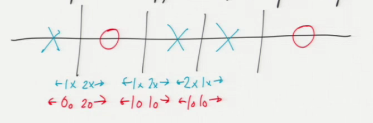
\includegraphics[scale=0.6]{images/binarysplits}
				\end{center}
			\end{itemize}
		\item Algorithms and running times:
			\begin{itemize}
				\item Test point: walk down tree until leaf. Return it's label.
				\begin{itemize}
					\item Worst-case time is $\mathcal{O}(\text{depth tree})$.
					\item For binary features, that's $\leq d$.
					\item Usually (not always) $\leq \mathcal{O}(\log n)$.
				\end{itemize}
				\item Training:
				\begin{itemize}
					\item For binary features, try $\mathcal{O}(d)$ splits at each node.
					\item For quantitative features, try $\mathcal{O}(n'd)$ splits; $n' =$ samples in node.
					\item Either way, $\Rightarrow \mathcal{O}(n'd)$ time at this node.
				\end{itemize}
				\item Each sample participates in $\mathcal{O}(\text{depth})$ nodes, cost $\mathcal{O}(d)$ time in each node.
				\item Running time $\leq \mathcal{O}(dn \text{depth})$.
			\end{itemize}
	\end{itemize}
	

\end{document}
